

\begin{savequote}[8cm]

  \qauthor{}
\end{savequote}



\chapter{\label{chap:trainingExperiment}Training experiment}

\minitoc


\section{Introduction}
The phenomenon of team click in joint action is widely substantiated by common intuition, anecdote, and ethnographic observation of group activities spanning sport to music/dance and even interactions in sedentary work place contexts.  The cognition of team click and its social effects remain poorly understood, however.  Often, the experience of team click is defined by a feeling of merely meeting expectations, but exceeding them---i.e., positively violation of expectations in joint action experienced as positive surprise or exhilaration.

The previous chapter presented empirical evidence of a relationship between perceptions of joint action success and social bonding, fully mediated by the phenomenon of team click.  The results of this naturalistic \textit{in situ} study are noteworthy as they provide evidence for the prediction that perceptions of joint action influence psychological processes of affiliation and connection with teammates, possibly via the mediating construct of team click.  A high stakes rugby tournament, however, contains many variables that may have confounded the specific relationships that are of interest in this dissertation.   Controlled experimental research is needed in order to more directly access causal mechanisms that underpin the relationship between joint action and social bonding.

Existing theory suggests that positive violation of expectation around joint action could be the source of feelings of team click and social bonding. How is it possible to experimentally manipulate conditions conducive to maximising this dimension of joint action? In addition, how is it possible to isolate joint action from other potential sources of information regarding the team and its performance such as explicit feedback from coaches and other players surrounding performance and joint action outcome?  This experimental study was designed with these considerations in mind.

These considerations lead to the hypothesis that expectations of higher levels of technical challenge in joint action will lead to higher levels of social bonding, due to the likelihood that athletes will experience more positive violations of expectations around team performance in the high-difficulty prime than in a low difficulty prime. It was predicted that the feeling of team click would mediate a relationship between positive violations of expectations and social bonding.  The predictions are outlined as follows:

The high difficulty prime was designed to encourage athletes to 1) generate lower expectations for individual and group performance, and 2) pay closer attention to the details of joint action between participants. It was therefore predicted that athletes in the high difficulty condition (more so than in the low difficulty condition) would report more positive perceptions of performance relative to prior expectations.

\begin{description}
\item[Prediction 1:] More positive perceptions of team performance relative to prior expectations will predict higher feelings of team click with the training group
\item[Prediction 1.a:] Violations of expectations around team performance will moderate the relationship between perceptions of joint action success and team click training among the training group
\item[Prediction 2:] Feelings of team click will positively correlate with feelings of social bonding to the training group
\item[Prediction 3:] More positive perceptions of team performance relative to prior expectations will predict higher levels of social bonding to the training group
\item[Prediction 4:] Feelings of team click will mediate a relationship between more more positive perceptions of group performance relative to prior expectations and social bonding to the group
\end{description}

A between-subjects experimental design was used, in which expectations of technical difficulty was manipulated in one of two conditions, ``high difficulty'' and ``low difficulty'' condition.  Surveys measuring athletes' perceptions of performance in joint action relative to prior expectations, feelings of team click, and feelings of social bonding to the specific training group were recorded both before and after the experiment.

%The closing of the introduction—typically the final paragraph or two—usually includes two important elements. The first is a clear statement of the main research question or hypothesis. This statement tends to be more formal and precise than in the opening and is often expressed in terms of operational definitions of the key variables. The second is a brief overview of the method and some comment on its appropriateness.

%These considerations lead to the hypothesis that the more bystanders to an emergency, the less likely, or the more slowly, any one bystander will intervene to provide aid. To test this proposition it would be necessary to create a situation in which a realistic “emergency” could plausibly occur. Each subject should also be blocked from communicating with others to prevent his getting information about their behavior during the emergency. Finally, the experimental situation should allow for the assessment of the speed and frequency of the subjects’ reaction to the emergency. The experiment reported below attempted to fulfill these conditions (p. 378).

%\subsection{Design}
%The design of a study is its overall structure. What were the independent and dependent variables? Was the independent variable manipulated, and if so, was it manipulated between or within subjects? How were the variables operationally defined?




Man Checks:
It was expected that athletes in the high difficulty condition would be less confident about their own and their group's ability to meet the technical challenges of the training session.  It was also predicted that athletes in the high difficulty condition would be more aroused than athletes in the low difficulty condition.
















\clearpage
\section{Method}

\subsection{Participants}
64 professional Chinese rugby players from two provincial programs were recruited for the study (men = 32, M(age) = 21.33 SD = 3.33, range = 16-29).  Athletes were recruited from two provincial rugby programs, 32
participants were athletes from Shandong province (men = 15, M(age) = 22.1) and the remaining 32 athletes were from Beijing province (men = 16, M(age) = 20.4).  This study was approved by the University of Oxford’s Central University Research Ethics Committee (SAME/CUREC1A/15-059).


\subsection{Materials}


\begin{figure}[htbp]
  \centering
      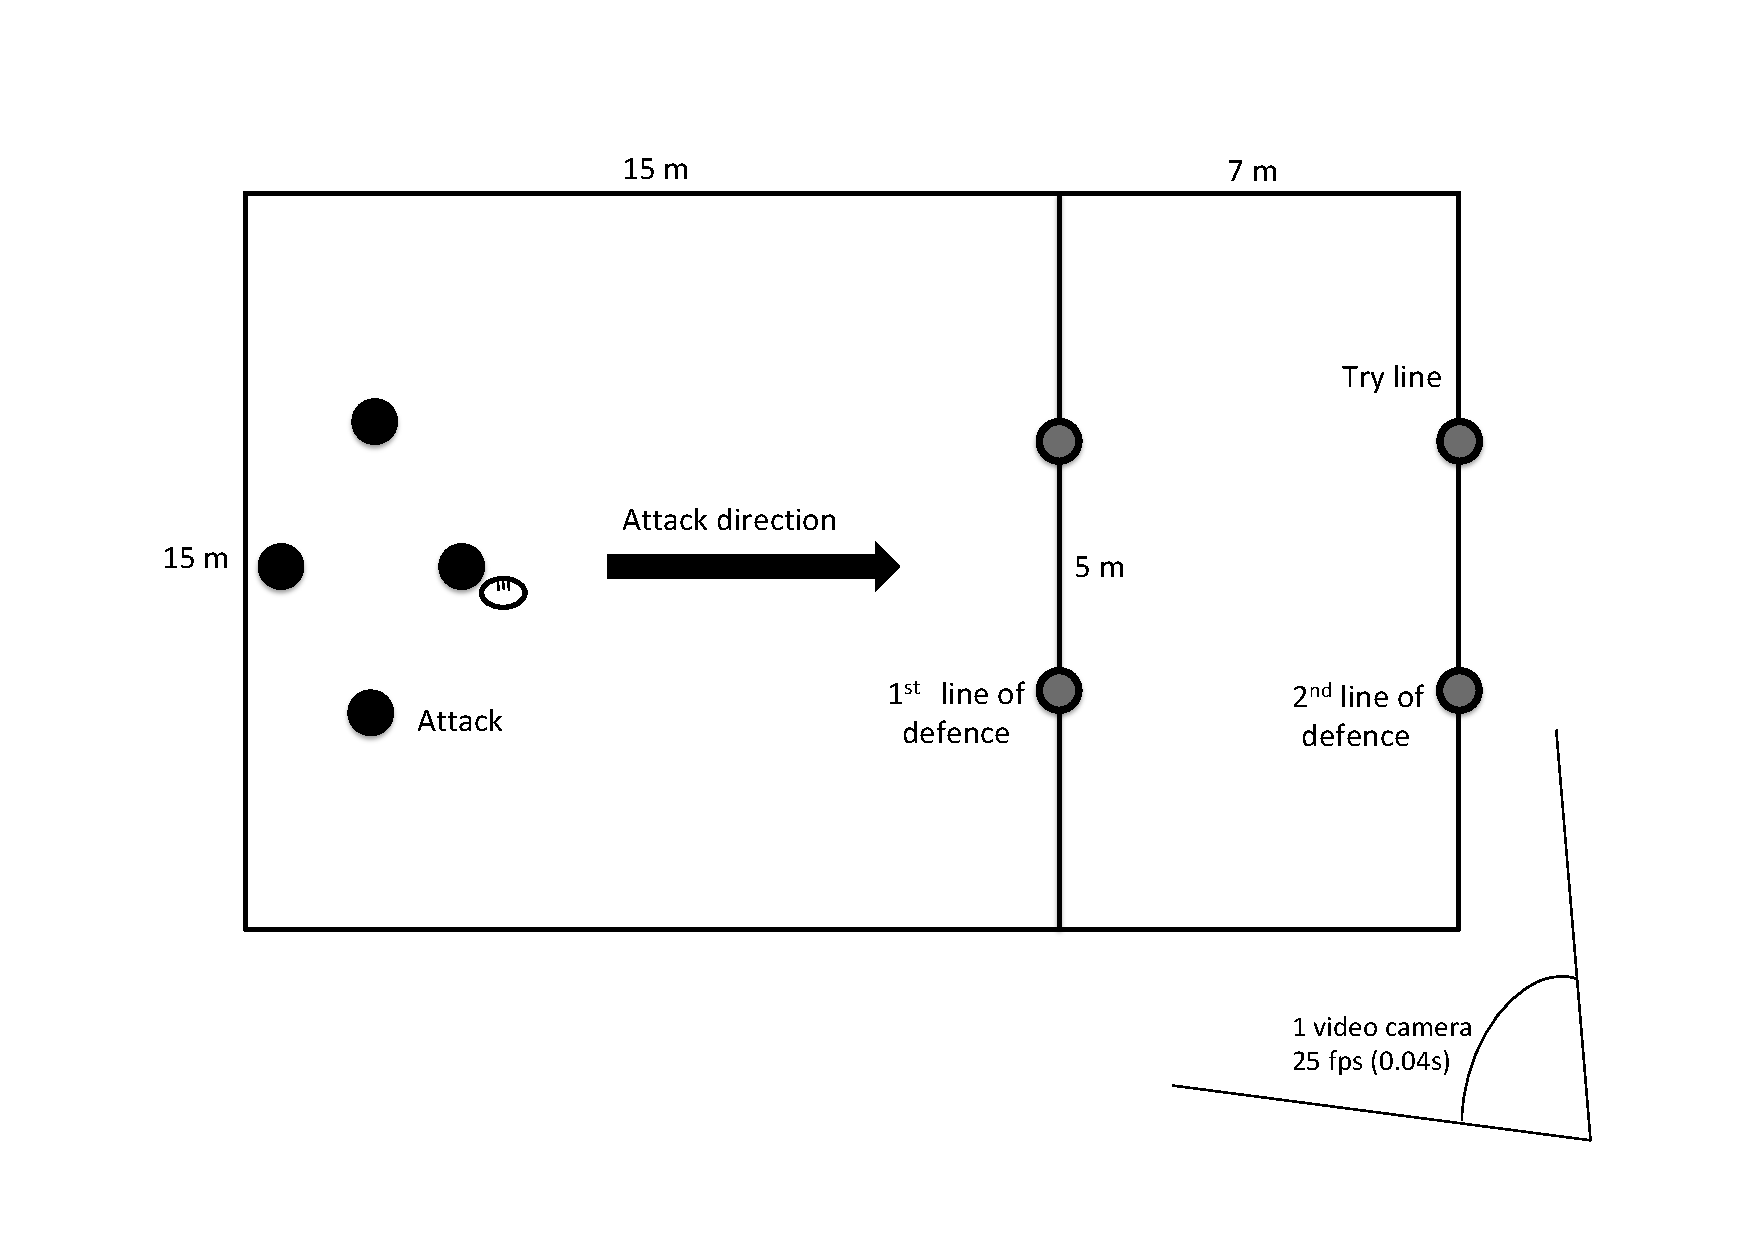
\includegraphics[width=0.9\linewidth,keepaspectratio] {images/invasionDrill}
      \caption{The Invasion Drill: a common training drill for rugby union in which a group of four attackers attempt to penetrate two consecutive lines of defence. Adapted from Passos (2011)}
      \label{fig:invasionDrill}
  \end{figure}


\subsubsection{Experimental Paradigm: The Invasion Drill}
This study required athletes to participate in a rugby training drill---known as ``Invasion Drill'' \citep{Biscombe1998}---which was preceded by one of two experimental primes—--a ``high difficulty'' condition, or a ``low difficulty'' condition.  This training drill was selected as it was representative of a typical subphase of joint action in rugby union and it has been successfully used to measure dynamic coupling between rugby players in joint action \citep[see][]{Passos2011}.  In this drill, a group of four rugby players form an attacking group and two pairs of opponents form a first and second defensive line.  The drill had two performance aims: (a) attackers were asked carry the ball into the try area, and (b) defenders were asked to stop the attacker’s progression toward the try line.
One trial consisted of one attempt by the attacking sub-group to penetrate two defending sub-groups, and carry the ball over the try line. The drill was conducted on a regulation multipurpose 110m x 70m grass or artificial turf training field within a 22m x 15m rectangle area marked by plastic cones (see Figure ~\ref{fig:invasionDrill}). The ball used was size 5, as recommended by World Rugby for this age group of athletes.\footnote{During my time conducting research and coaching in China, I did not commonly witness the Invasion Drill as described herein in training scenarios. As such, I judged that the Invasion Drill would be suitable for this experiment because the technical requirements of the drill were be suitably familiar to athletes (i.e., a typical subphase of joint action in rugby), but the drill itself would be suitably novel.}


%The training drill, known as ``Invasion Drill,'' requires eight athletes, one sub-grouof four attackers and two sub-groups of two defenders.  The primary aim of the drill is for the sub-group of 4 attacking players to successfully penetrate two consecutive lines of two defenders (also commonly known as a ``4 on 2 + 2'' drill). The aim of the two defending sub-groups is to stop the attacking team from achieving the primary goal, by interfering with their coordination by halting the ball-carrier, or the ball in flight between attacking players.


\subsubsection{Experimental Conditions: high and low difficulty\label{sect:expPrimes}}
Two different experiment primes were developed in order to manipulate athletes’ expectations around the technical difficulty of the impending joint-action task.  Athletes in the ``high difficulty'' condition learned that the overall average difficulty rating for the training drill, provided by World Rugby coaches and athletes, was 77.5/100, or approximately 8 out of 10.  Athletes were told that the drill would require an extension of their abilities as individuals and as a training group.  By contrast, athletes in the ``low difficulty'' condition learned that they would be participating in an ostensibly different drill with an overall average difficulty rating of 22.5/100, or approximately 2 out of 10 (see Appendix~\ref{app9:conditionPrime} for full script).  In reality, the training drill was exactly the same for all experimental sessions.  Based on a pilot study with 20 athletes from the Beijing men's and women's rugby programs who did not participate in the study, the actual difficulty of this drill was estimated to be approximately 5/10 (see Appendix~\ref{app9:difficultyPilot} for full explanation of pilot study).  The experiment primes were designed to encourage athletes to either over or under rate the difficulty of the impending training drill. If successful, the prime would alter athletes' expectations around certainty of performance, such that athletes in the high difficulty condition would enter the training drill with expectations for performance that were on average lower than athletes in the low difficulty prime. It was predicted that athletes in the high difficulty condition would experience more positive perceptions of group performance relative to prior expectations, as compared to athletes in the low difficulty condition, who would on average experience experience less positive violations of expectations around group performance.


\subsubsection{Measures}


\myparagraph{Surveys}
Surveys were administered at three time points: Baseline ( approximately 24 hours before the experiment), Pre-Drill (immediately before the training drill and after receiving the experiment prime), and Post-Drill (immediately following the completion of the drill; see ~\ref{tab:surveyMeasureSummaryTable}). Consistent with the previous study (Chapter~\ref{chap:tournamentSurvey}), athletes responded to questions about 1) \textit{performance} (including perceptions of individual and team performance relative to prior expectations, and perceptions of components of individual and team performance), 2) \textit{team click} (feelings associated with team click in joint action), and (3)\textit{social bonding} (feelings of social bonding and group membership).  Additionally, athletes responded to questions designed to measure \textit{moderator variables} such as technical competence, personality type, injury status, arousal, and fatigue. Measures of athlete confidence in group and self to meet the technical challenges of the Drill and physiological arousal would be used to check the experimental manipulation (see Section~\ref{sec:manChecksDrill}).


    % Please add the following required packages to your document preamble:
% \usepackage{booktabs}
\begin{table}[]
\centering
\begin{tabular}{@{}rlcc@{}}
\toprule
\multicolumn{1}{c}{Items} & \multicolumn{1}{r}{Baseline} & Pre-Drill & Post-Drill \\ \midrule
\multicolumn{1}{c}{\textbf{Training Group}} & \multicolumn{1}{r}{} &  &  \\ \midrule
\begin{tabular}[c]{@{}r@{}}Confidence in group \\ to meet technical \\ challenges\end{tabular} &  & \cmark & \multicolumn{1}{l}{} \\
\multicolumn{1}{l}{} &  & \multicolumn{1}{l}{} & \multicolumn{1}{l}{} \\
\begin{tabular}[c]{@{}r@{}}Group performance \\ vs prior expectations\end{tabular} & \multicolumn{1}{r}{} &  & \cmark \\
\multicolumn{1}{l}{} &  & \multicolumn{1}{l}{} & \multicolumn{1}{l}{} \\
\begin{tabular}[c]{@{}r@{}}Components of \\ performance\end{tabular} & \multicolumn{1}{r}{} & \cmark & \cmark \\
\multicolumn{1}{l}{} &  & \multicolumn{1}{l}{} & \multicolumn{1}{l}{} \\
Team Click &  & \cmark & \cmark \\
\multicolumn{1}{l}{} &  & \multicolumn{1}{l}{} & \multicolumn{1}{l}{} \\
Social Bonding &  & \cmark & \cmark \\ \midrule
\multicolumn{1}{c}{\textbf{Individual}} &  & \multicolumn{1}{l}{} & \multicolumn{1}{l}{} \\ \midrule
\begin{tabular}[c]{@{}r@{}}Confidence in self\\ to meet technical \\ challenges\end{tabular} &  & \cmark & \multicolumn{1}{l}{} \\
\multicolumn{1}{l}{} &  & \multicolumn{1}{l}{} & \multicolumn{1}{l}{} \\
\begin{tabular}[c]{@{}r@{}}Individual performance\\  vs prior expectations\end{tabular} &  & \multicolumn{1}{l}{} & \cmark \\
\multicolumn{1}{l}{} &  & \multicolumn{1}{l}{} & \multicolumn{1}{l}{} \\
\begin{tabular}[c]{@{}r@{}}Components of \\ individual performance\end{tabular} & \multicolumn{1}{r}{\cmark} & \cmark & \cmark \\ \midrule
\multicolumn{1}{c}{\textbf{Team (Province)}} & \multicolumn{1}{r}{} &  &  \\ \midrule
Team Performance & \multicolumn{1}{r}{\cmark} &  & \cmark \\
\multicolumn{1}{l}{} &  & \multicolumn{1}{l}{} & \multicolumn{1}{l}{} \\
Team Click & \multicolumn{1}{r}{\cmark} &  & \cmark \\
\multicolumn{1}{l}{} &  & \multicolumn{1}{l}{} & \multicolumn{1}{l}{} \\
Social Bonding & \multicolumn{1}{r}{\cmark} &  & \cmark \\ \midrule
\multicolumn{1}{c}{\textbf{Moderators}} &  & \multicolumn{1}{l}{} & \multicolumn{1}{l}{} \\ \midrule
Arousal & \multicolumn{1}{r}{} & \cmark & \cmark \\
Exertion & \multicolumn{1}{r}{} &  & \cmark \\
Injury & \multicolumn{1}{r}{} & \cmark & \cmark \\
Personality & \multicolumn{1}{r}{\cmark} &  &  \\
Technical competence & \multicolumn{1}{r}{\cmark} &  & 
\end{tabular}
\caption{Survey items measured at Baseline, Pre-Drill, and Post-Drill.}
\label{tab:surveyMeasureSummaryTable}
\end{table}


\myparagraph{Baseline}
Baseline measures were obtained 24 hours before the start of the experiment by asking athletes about their impressions of recent individual performance and the performance of their provincial squad as a whole.  Survey items included questions relating to specific components of team and individual performance (e.g., team components: attack, defence, on-field communication, and support play; individual components: passing technique, one-on-one tackling, effectiveness in contact areas), as well as items relating to overall impressions of performance, for example: ``How well do you feel your team has been performing in training and competition over the past month?'' (100 point scale, 0 = ``Extremely bad'', 100 = ``Extremely good'').  Athletes also responded to questions about feelings of team click and social bonding with their team as a whole.  In addition, the Baseline survey also included items concerning basic personal information, current injury status, subjective and objective measures of technical competence, and personality type.  For a full explanation of the Baseline survey, see Appendix ~\ref{app9:trainingExperiment} Section ~\ref{app9:surveyItemsBaseline}.


\myparagraph{Pre-Drill}
Immediately before each experiment session, athletes were asked questions about feelings and expectations concerning their individual performance and the performance of their specific training group in the impending training drill.  For example, athletes were asked ``How do you feel \textit{right now} about your individual performance'' (100 point scale, 0 = ``Extremely bad'', 100 = ``Extremely good'').  Athletes also responded to items asking about confidence in self and the training group to meet the technical challenges of the drill, i.e. ``How confidence are you in your own / your training group's ability to meet the technical challenges of the upcoming drill'' (100 point scale, 0 = ``Not at all confident'', 100 = ``Extremely confident'').

Athletes were also asked a series of questions about feelings of team click and social bonding to their specific training group. For team click, for example, athletes were asked questions like: ``How do you feel the tacit understanding is between the training group today?'' (100 point scale, 0 = ``Extremely bad'', 100 = ``Extremely good'').  For social bonding, athletes were asked questions like: ``How emotionally supportive does your training group feel right now?'' (100 point scale, 0 = ``Extremely weak'', 100 = ``Extremely strong'').

%See Appendix~\ref{app9:surveyItemsPre} for an outline of the Pre-Drill survey.

\myparagraph{Post-Drill}
Immediatley upon completion of the drill, athletes responded to questions concerning their impression of their individual performance and the performance of their training group in the training drill. A  single item measure asked about individual and group performance relative to prior expectations: ``Overall, how do you feel about your training group's performance in training today?'' (100 point scale, 0 = ``Much worse than expected'', 100 = ``Much better than expected'').  Athletes were also asked about their feelings team click and group bonding to the training group, e.g.

In addition, athletes were asked to answer survey items designed to measure social bonding to the provincial team as a whole (these team-focussed questions replicated the survey items that were asked one day earlier at Baseline).  See Appendix ~\ref{app9:trainingExperiment} Section ~\ref{app9:surveyItemsPost} for an outline of the Post-Drill survey.
%~\ref{} Section ~\ref{}.

Surveys were designed and administered using Qualtrics software (Qualtrics version 9, Provo, UT). The surveys (initially designed in English) were translated into modern Chinese by the researcher and back translated by two independent native Chinese speaking translators from Beijing Sports University to verify accuracy.  Athletes completed the modern Chinese version of each survey using WeChat on their personal mobile devices connected remotely to the internet. Survey data were processed and analysed using the R environment (R Development Core Team, 2006).

\subsubsection{Video analysis of training group performance in training drill\label{sec:videoAnalysis}}
In order to produce quantitative measures of interpersonal coordination between co-actors, athletes’ motion was captured by a single digital video camera (Sony FDR-AX700 4K HDR Camcorder) mounted on a 1.2m high tripod.

The digital camera and tripod were positioned on a platform 2m above the level of the playing field, approximately 10-15m from the bottom try-line corner of the Invasion Drill perimeter (see Figure ~\ref{fig:invasionDrill}). The experimenter began video recording before the athletes arrived, and ceased recording after all athletes had left the training field following the experiment. Digital video images of action were acquired by a computer and files were saved on an encrypted external hard disk in .AVI format.

%For image treatment, TACTO 8.0 software was used for digitising at 25 frames per second.

Video footage from all 8 experiment sessions was analysed by the researcher as well as an hypothesis blind research assistant familiar with the sport of rugby.  Each experimental trial of the Invasion Drill (16 in total) was coded according to success of the group in the primary (attacking) goal of the drill, i.e., scoring a try by carrying the ball over the try line.  Two measures were constructed: a binary try or no try (``Try''; 1 = ``try'', 0 = ``no try'') measure, and a measure designed to reflect the quality of the outcome of each trial (``Trial Outcome''). For this second and more fine-grained measure, a maximum value of 6 was awarded to a ``clear try'' (trials in which a clear unobstructed try was scored by the attacking sub-unit); 5 to a ``rough try'' (the ball-carrier crossed the try-line following some minimal level of physical contact or obstruction from the defence that did not halt the momentum of the attacking phase); 4 to an ``Obstructed try'' (a trial in which a try is scored, but the momentum of the attacking sub-unit was clearly interrupted); 3 to a ``no try - defence'' (a trial in which a ball carrier is completely obstructed by a defender, and the trial is unsuccessful largely due to the effectiveness of the defence); 2 to a ``no try - defence forced error'' (unsuccessful trial due to a combination of the defence and error in attack); 1 to a ``no try - unforced error'' (a failed trial due to an unforced error in attack, such as an athlete passing the ball forward, or dropping the ball without obvious pressure from the defence).  For each experiment session of 16 trials, the total number of successful trials was calculated (``Tries Total''), as well as the average quality of performance outcome (``Trial Outcome Average'').

%In addition, the the standard deviation of this mean outcome (``Trial Outcome SD'') was calculated in order to capture the variance of performance for each training group.

The researcher briefed the hypothesis blind research assistant using 10 trials randomly selected from the warm-up trials of each experiment session. Owing this detailed briefing and the research assistant's familiarity, inter-rater reliability, measured using Cohen's (1960) kappa \citep[suitable for two coders, see][]{DiEugenio2004} was high for both the Try ($\kappa = .96, Z(128) = 10.60, p < .001$) and Trial Outcome ($\kappa = .90, Z(128) = 18.96, p < .001$), suggesting almost perfect agreement.

\subsection{Procedure}
Permission to run the study was sought from the head coach of each of the four teams (Beijing men's, Beijing women's, Shandong men's, Shandong women's).  These coaches nominated athletes who were fit and able to complete the session without compromising their existing training schedules.  Athletes were randomly assigned to one of two conditions, and then to a particular experimental group, with some subsequent adjustments to assignments to ensure that each condition was matched as much as possible according to average training age.  Once athletes were assigned to an experiment group, they were then added to a WeChat group populated by other training group members and the researcher.

\myparagraph{Cover Story}
Athletes were notified (first via WeChat and then in a team meeting) that they were due to participate in a trial of a various rugby training drills selected from a recent World Rugby report on training methods for rugby sevens.  Athletes were told that the training drills had been previously rated by a selection of international level coaches and players from all over the world (including Asia and China).  Athletes were informed that the purpose of the exercise was to assess the ratings provided by World Rugby (the international governing body of rugby union) by replicating these drills with more rugby athletes in China.  Athletes were told that survey measures and video footage would be collected, which would be used to analyse individual performance of athletes in each training drill.

%%It was also explained to athletes that there would be a second round of drills also requiring groups of eight athletes, but the makeup of training groups for these groups may reshuffle depending on athletes preferences following the first round of drills.  This detail allowed for the inclusion of a Post-Drill bonding measure, in which athletes were asked to what extent they wished to continue to train with the same 8-athlete training group in a subsequent round of drills.

\myparagraph{Baseline survey}
Approximately 24 hours before the experiment session, athletes were instructed to complete the baseline survey by opening a link provided in the WeChat group.  This survey included formal consent for the study.  Approximately 1 hour before the experiment was due to take place, athletes received a notification in WeChat including information about the projected difficulty of their impending drill session (the experimental prime, for either the ``high difficulty'' or ``low difficulty'' conditions (see Section ~\ref{sect:expPrimes} for detailed descriptions).   All athletes were lead to believe that athletes in the other experiment groups were performing different drills to their assigned drill.  In reality, the training drill for each condition was identical, the only thing that varied was the prime administered before the drill.

\myparagraph{Pre-Drill survey}
Once the 8 athletes participating in the experiment session were all assembled at the designated training field, the researcher verbally re-administered the same prime that had been sent earlier to the athletes via WeChat, and athletes were told in more detail about the requirements of the Invasion Drill.  For example, athletes learned that they would be assessed based on their performance in attack, defence, and their ability to coordinate attack and defence with others (to be assessed through subsequent video analysis).  Athletes were provided with no other explicit information regarding performance goals, besides completing the drill to the best of their ability within the rules of rugby.

%Specifically, athletes were told that their performance in the experiment would be assessed based on subsequent video analysis.

Athletes were then given the Pre-Drill survey, which took approximately four minutes to complete.  After all the athletes finished the survey, they participated in a standard warm up routine lasting approximately 10 minutes, including slow jogging and dynamic stretching.  Athletes were instructed not to use the rugby ball during this period, which served to reduce the amount of incidental coordination and interaction between participants prior to the start of the experiment trials.  Following the warm up, the group assembled in the training drill area.  One athlete was randomly assigned to stand at each of eight available plastic markers.  In this position, athletes were told once more about the structure and procedure for the training drill, in particular the way in which athletes were expected to rotate clockwise after every trial of the drill so that athletes did not habituate to occupying certain positions or coordinating within certain sub-units in the drill.

\myparagraph{Invasion drill}
To begin the drill, the ball-carrier at the front and centre of the attack sub-group was instructed to tap the ball with his/her foot, before initiating the attacking sub-phase by advancing forward towards the defence sub-units.  In the case that the ball was immediately fumbled during the initiation of the trial, the training group was instructed to restart that trial and the trial in which the mistake was made was not counted.  Following a block of 4 practice trials, athletes were told by the researcher that the formal test was beginning.  The group of athletes then completed 16 trials of the drill, which allowed each athlete to complete four trials of attack and four trials of defence, in different positions.


\myparagraph{Post-Drill survey}
Following completion of all 16 test trials, athletes assembled and were thanked for their participation.  Athletes were then instructed to go directly to the side of the field to complete the final Post-Drill survey using their mobile devices.

%Following the completion of this final survey, athletes were told that they would be informed within two days about the next drill (in fact, no more drills were taking place).

%\myparagraph{Video Analysis Procedure}
%The digital camera and tripod were positioned on a platform 2m above the level of the playing field, approximately 10-15m from the bottom try-line corner of the Invasion Drill perimeter (see figure ~\ref{fig:invasionDrill}).  The experimenter began video recording before the athletes arrived, and ceased recording after all athletes had left the training field following the completion of the drill.  Digital video images of action were acquired by a computer, using a USB2.0 cable, and files were saved on an encrypted external hard disk in .AVI format.

%For image treatment, TACTO 8.0 software was used for digitizing at 25 frames per second.
%The procedure is how the study was carried out. It often works well to describe the procedure in terms of what the participants did rather than what the researchers did. For example, the participants gave their informed consent, read a set of instructions, completed a block of four practice trials, completed a block of 20 test trials, completed two questionnaires, and were debriefed and excused.

\clearpage
\section{Data analysis}

\subsection{Data reduction}
Exploratory factor analysis (EFA) was used to reduce multicolinearity between variables while retaining as much variance as possible in the observed data \citep[, see Appendix~\ref{app5:EFA}]{Yong2013}. EFA followed the procedure outlined in the previous empirical chapter (see Chapter~\ref{tournamentSurvey} Section~\ref{Ch5:dataReduction}).
EFAs were performed on clusters of survey items pertaining to performance, team click, and social bonding, directed at both the training group and the athlete's provincial team as a whole.  Moderator variables---technical competence (objective and subjective), components of individual and training group performance, arousal, fatigue, and athlete perception of team discipline---were also reduced to factors. Due to the equivalence of measures between Pre- and Post-Drill surveys, EFAs were conducted on the entire available data (rather than separate EFAs for the Post-Drill and Pre- to Post-Drill subsets).

%The only exception to this procedure was


%(see Appendix~\ref{app9:dataReduction} for full description)
%In addition, items relating to team click and social bonding directed at the provincial team as a whole (and not just the specific training group) were reduced to factors, in order to assess pre- to post-experiment variation in generalised bonding to the team.

\myparagraph{Perceptions of group and individual performance relative to prior expectations}
The main predictor variable of interest, perceptions of training group performance relative to prior expectations, was a single item measure, and did not require data reduction.  Given that most outcome variables of interest were factors standardised as z-scores (with $mean = 0, SD = 1$), perceptions of group performance relative to prior expectations was also transformed to a standardised z-score so as to accord with explanatory variables in subsequent subsequent linear mixed effects modelling \citep[for an explanation, see, for example, ][1058]{Beckmann2003}.


\subsection{Data structure}
Study predictions were tested by analysing two data sets:  1) Post-Drill survey data and 2) variation between Pre- and Post-Drill survey data.  Linear mixed effects regression (LMER) models (package \textit{lme4} in the R environment) were used to test relationships between variables of interest, owing to their ability to model the random structure of the data (see Chapter~\ref{tournamentSurvey} Section ~\ref{survey:survey:dataStructureModelSelection} for full explanation).  Unless otherwise stated, all models controlled for the average performance outcome of each trial (Trial Outcome Average), subjective and objective measures of athlete technical competence, personality (extraversion), and arousal measured Post-Drill.  Intra-class correlation (ICC) estimates were calculated to account for clustering of model residuals according to groupings of athlete sex, team, and specific experiment session. ICC values of $>.10-20$ were considered meaningful, and informed which random structure to specify in LMER models.

%Results from models of each data set are reported according to study predictions in Section ~\ref{sect:resultsStudyPredictions}.

\myparagraph{Mediation analyses}
Mediation analyses were conducted using linear mixed effects regressions in the Causal Mediation Analysis package in R (Version 4.4.5).  To make inferences concerning the average indirect and total effects, quasi-Bayesian Markov Chain Monte Carlo (MCMC) method based on normal approximation and 1000 simulations was used to estimate the 95\% Confidence Intervals \citep{Tofighi2016a,Imai2010}. MCMC estimation is a form of non-parametric bootstrapping whereby the sampling distribution for the effect of interest is not assumed to be normal but is instead simulated from the model estimates and their asymptotic variances and covariances \cite{Preacher2008}.

%Moderated mediation occurs when either path a (group performance to team click) or path b (from team click to bonding), or both are moderated \citep{Edwards2007,Hayes2017}


\subsection{Manipulation Checks\label{sec:manChecksDrill}}
Three survey items administered immediately following the researcher's in-person delivery of the experimental prime and immediately before the training drill were designed to test the effectiveness of the experimental manipulation.  Athletes were asked to report:

\begin{enumerate}
  \item Confidence in individual ability to meet the technical challenges of the training drill
  \item Confidence in training group's ability to meet the technical challenges of the training drill
%  \item Physiological arousal (see Appendix ~\ref{app5:tournamentSurvey} Section ~\ref{app5:exertionMid} for full details)
\end{enumerate}

Athlete responses to these items were compared according to experiment condition using LMER to model the random structure of the data, and controlling for technical competence.


































\clearpage
\section{Results}


\subsection{Descriptive Statistics \label{sec:descriptives}}

\subsubsection{Participants}
58 athletes ($men = 31, M(age) = 21.33 SD = 3.33, range = 16-29$) participated in the experiment in groups of eight (or on two occasions six).  A total of eight experimental sessions were conducted, with participants each taking part in a session only once.  31 participants were from Shandong province ($men = 15, M(age) = 22.1$) and the remaining 27 athletes were from Beijing province ($men = 16, M(age) = 20.4$).  The experimental groups consisted of athletes from the same province. On three separate occasions (in Shandong province), a dummy participant stood in for an athlete who failed to attend due to injury or illness.  In all three instances, dummy participants were competent ex-athletes who were naive to the predictions of the study, and did not participate in the pre- or post-drill surveys. For both experiment trials with the Beijing women's team, only 11 athletes were available to participate in the two sessions.  As a compromise, both drills were modified to become ``$3+2+1$'' (in the session with only five fit athletes, a research assistant participated as dummy assistant).  Survey data of the remaining 58 participants (and video data of all 64 athletes, including dummy participants) were analysed.

% latex table generated in R 3.5.0 by xtable 1.8-2 package
% Wed May 16 15:48:41 2018
\begin{table}[ht]
\centering
\begin{tabular}{rlll}
  \hline
 & Overall & high & low \\ 
  \hline
n &    58 &    29 &    29 \\ 
  Age (mean (sd)) & 21.33 (3.33) & 20.48 (3.11) & 22.14 (3.39) \\ 
  Sex = male (\%) &    31 (53.4)  &    15 (51.7)  &    16 (55.2)  \\ 
  \textbf{Team} (\%) &     &     &     \\ 
     Beijing Men &    16 (27.6)  &     8 (27.6)  &     8 (27.6)  \\ 
     Beijing Women &    11 (19.0)  &     6 (20.7)  &     5 (17.2)  \\ 
     Shandong Men &    15 (25.9)  &     7 (24.1)  &     8 (27.6)  \\ 
     Shandong Women &    16 (27.6)  &     8 (27.6)  &     8 (27.6)  \\ 
  Position = Starting Team (\%) &    18 (32.7)  &     9 (33.3)  &     9 (32.1)  \\ 
  TrainingAge (mean (sd)) &  4.22 (2.11) &  3.74 (1.89) &  4.68 (2.25) \\ 
  YearsInTeam (mean (sd)) &  5.64 (2.08) &  5.37 (1.94) &  5.89 (2.20) \\ 
  \textbf{AthleteLevel} (\%) &     &     &     \\ 
     1st Level &    11 (20.8)  &     5 (19.2)  &     6 (22.2)  \\ 
     2nd Level &     6 (11.3)  &     5 (19.2)  &     1 ( 3.7)  \\ 
     Master &    36 (67.9)  &    16 (61.5)  &    20 (74.1)  \\ 
  \textbf{ContractStatus} (\%) &     &     &     \\ 
     Full time contract &     8 (14.5)  &     3 (11.1)  &     5 (17.9)  \\ 
     Full time employee &    21 (38.2)  &    10 (37.0)  &    11 (39.3)  \\ 
     Student contract &     8 (14.5)  &     5 (18.5)  &     3 (10.7)  \\ 
     Training contract &    16 (29.1)  &     8 (29.6)  &     8 (28.6)  \\ 
     Trial status &     2 ( 3.6)  &     1 ( 3.7)  &     1 ( 3.6)  \\ 
   \hline
\end{tabular}
\caption{Overview of experiment sample (overall and by condition).} 
\label{tab:athleteDescriptivesTrainingOverall}
\end{table}


Basic information concerning participants is displayed in Table ~\ref{tab:athleteDescriptivesTrainingOverall}.  Athletes' average training age (years dedicated to full-time rugby training) was 4.22 years ($SD = 2.11$), and athletes had spent an average of 5.64 years ($SD = 2.08$) in the team.  50\% of the sample (29) were either full-time employees of their provincial team (21), or were otherwise employed on a full-time (but fixed term) contract (8).  The remaining 29 athletes were employed either on a ``student contract'' (8 or 14.5\%), or on a short term training contract (16 or 29.1\%), or on a short-term trial basis (2 or 3.6\%).  18 athletes (31\%) declared that there were in the starting team of their respective teams.

%\footnote{Being a member of the starting team indicated that athletes were among the most (if not the most) competent athletes in their position in their team.}
All athlete attributes mentioned above appeared to be evenly matched between conditions, except for key variables of athlete age and training age, which appeared to be higher in the low difficulty condition than in the high difficulty condition. Independent-sample t-tests were conducted to compare key variables of athlete training age and athlete age in the high and low difficulty conditions. There was a significant difference in athlete age in between the high ($M= 20.48(SD =3.11)$) and low ($M= 22.14(SD =3.39)$) difficulty conditions; $t(52.09) = -3.3279, df = 162.59, p-value = 0.001$.  The difference in training age between high ($M= 3.74 (SD =1.90)$) and low ($M= 20.48(SD =2.25)$) difficulty conditions, was not significant $t(52.09)= -1.67, df = 162.59, p-value = 0.10$, but indicated a marginally significant trend.

%(see Table ~\ref{tab:athleteDescriptivesTrainingOverall}).



\subsubsection{Key variables of interest \label{sec:surveyResponses}}

Main variables of interest relating to performance (both objective performance outcome and survey items), team click, and social bonding (to the training group and provincial team) are collated by condition (high/low) time point (Baseline, Pre-Drill, Post-Drill) in see Table ~\ref{tab:rawPerformance} and ~\ref{tab:rawClickBond}. In general, the central tendency of all survey items was between .5 to 1.5 standard deviations above the mid-point of the scale (50 for 100 points scales such as Tacit Understanding or Emotional Support, or 2.5 for the Fusion and Group Identity scales.   For instance, central tendencies of variables measuring athletes' perceptions of team click and social bonding ranged from a low of 68.34 ($SD = 14.69$) for feelings of tacit understanding measured Post-Drill in the low difficulty condition, to a high of 90.21 ($SD = 9.33$) for feelings of shared goal with the training group measured Pre-Drill in the low difficulty condition.

Athletes were on average more critical in regards to perceptions of individual performance than they were of group and team performance, and were generally more critical of individual and group performance in the Post-Drill survey than they were in the Baseline and Pre-Drill surveys.  Measures relating to Team Click and Social bonding appeared to decrease in the Post-Drill survey relative to the Pre-Drill and Baseline surveys. Confidence in self and the training group to meet the challenges of the training drill did not appear to vary according to condition.

Objective performance outcome did appear to vary, with the low difficulty experiment sessions averaging 11.83 ($SD = .85$) tries and the high condition only 8 ($SD = 2.20$) tries (the most successful tries scored in an experiment session was 13, while the lowest amount of tries scored in an experiment session was 4).  For the more fine grained performance score, ``Trial Outcome Average'' the average for the low difficulty condition was 4.68 ($SD = .25$), while the average for the high difficulty condition was 3.52 ($SD = .49$). A more detailed report of performance outcome by experiment session is shown in Table ~\ref{tab:trainingObjPerformanceSession}.  For a description of additional variables, including moderator variables, see Appendix~\ref{app9:descriptives}.

% Please add the following required packages to your document preamble:
% \usepackage{booktabs}
\begin{table}[]
  \centering
  \begin{tabular}{@{}rcccccc@{}}
\toprule
\multicolumn{1}{c}{\textbf{Performance Item}} & \multicolumn{2}{c}{\textbf{Baseline}} & \multicolumn{2}{c}{\textbf{Pre}} & \multicolumn{2}{c}{\textbf{Post}} \\ \midrule
\multicolumn{1}{c}{\textbf{}} & High & Low & High & Low & High & Low \\
\textbf{Objective Performance} & \multicolumn{1}{l}{} & \multicolumn{1}{l}{} & \multicolumn{1}{l}{} & \multicolumn{1}{l}{} & \multicolumn{1}{l}{} & \multicolumn{1}{l}{} \\
Tries Total & \multicolumn{1}{l}{} & \multicolumn{1}{l}{} & \multicolumn{1}{l}{} & \multicolumn{1}{l}{} & \begin{tabular}[c]{@{}c@{}}8.00 \\ (2.20)\end{tabular} & \begin{tabular}[c]{@{}c@{}}11.83 \\ (.85)\end{tabular} \\
\begin{tabular}[c]{@{}r@{}}Trial Outcome \\ Average\end{tabular} & \multicolumn{1}{l}{} & \multicolumn{1}{l}{} & \multicolumn{1}{l}{} & \multicolumn{1}{l}{} & \begin{tabular}[c]{@{}c@{}}3.52 \\ (.49)\end{tabular} & \begin{tabular}[c]{@{}c@{}}4.68\\ (.25)\end{tabular} \\
\multicolumn{1}{l}{} & \multicolumn{1}{l}{} & \multicolumn{1}{l}{} & \multicolumn{1}{l}{} & \multicolumn{1}{l}{} & \multicolumn{1}{l}{} & \multicolumn{1}{l}{} \\
\textbf{Training Group} &  &  &  &  &  &  \\
\begin{tabular}[c]{@{}r@{}}Confidence in group \\ to meet technical \\ challenges\end{tabular} & - & - & \begin{tabular}[c]{@{}c@{}}76.03 \\ (17.16)\end{tabular} & \begin{tabular}[c]{@{}c@{}}78.62\\ (12.75)\end{tabular} & - & - \\
\multicolumn{1}{l}{} &  &  &  &  &  &  \\
\begin{tabular}[c]{@{}r@{}}Performance vs \\ prior expectations\end{tabular} & - & - & - & - & \begin{tabular}[c]{@{}c@{}}66.50 \\ (20.64)\end{tabular} & \begin{tabular}[c]{@{}c@{}}66.83 \\ (18.32)\end{tabular} \\
\multicolumn{1}{l}{} &  &  &  &  &  &  \\
Components: &  &  &  &  &  &  \\
Attack & - & - & \begin{tabular}[c]{@{}c@{}}74.55 \\ (20.93)\end{tabular} & \begin{tabular}[c]{@{}c@{}}75.66 \\ (13.36)\end{tabular} & \begin{tabular}[c]{@{}c@{}}64.07 \\ (24.38)\end{tabular} & \begin{tabular}[c]{@{}c@{}}67.34 \\ (15.61)\end{tabular} \\
Defence & - & - & \begin{tabular}[c]{@{}c@{}}73.38 \\ (22.09)\end{tabular} & \begin{tabular}[c]{@{}c@{}}77.62 \\ (14.44)\end{tabular} & \begin{tabular}[c]{@{}c@{}}57.04 \\ (25.55)\end{tabular} & \begin{tabular}[c]{@{}c@{}}63.14 \\ (19.90)\end{tabular} \\
On-field communication & - & - & \begin{tabular}[c]{@{}c@{}}77.76 \\ (16.09)\end{tabular} & \begin{tabular}[c]{@{}c@{}}75.72 \\ (14.84)\end{tabular} & \begin{tabular}[c]{@{}c@{}}66.25 \\ (20.78)\end{tabular} & \begin{tabular}[c]{@{}c@{}}70.66 \\ (15.46)\end{tabular} \\
Support Play & - & - & \begin{tabular}[c]{@{}c@{}}77.55 \\ (15.65)\end{tabular} & \begin{tabular}[c]{@{}c@{}}75.97 \\ (12.80)\end{tabular} & \begin{tabular}[c]{@{}c@{}}64.46 \\ (25.32)\end{tabular} & \begin{tabular}[c]{@{}c@{}}69.66 \\ (13.72)\end{tabular} \\
\multicolumn{1}{l}{} &  &  &  &  &  &  \\
\textbf{Individual} &  &  &  &  &  &  \\
\begin{tabular}[c]{@{}r@{}}Confidence in self\\ to meet technical \\ challenges\end{tabular} & - & - & \begin{tabular}[c]{@{}c@{}}76.90 \\ (22.65)\end{tabular} & \begin{tabular}[c]{@{}c@{}}77.76 \\ (15.37)\end{tabular} & - & - \\
\multicolumn{1}{l}{} &  &  &  &  &  &  \\
\begin{tabular}[c]{@{}r@{}}Overall impression \\ of individual performance\end{tabular} & \begin{tabular}[c]{@{}c@{}}69.07 \\ (18.62)\end{tabular} & \begin{tabular}[c]{@{}c@{}}66.11 \\ (19.47)\end{tabular} & \begin{tabular}[c]{@{}c@{}}65.66 \\ (27.57)\end{tabular} & \begin{tabular}[c]{@{}c@{}}69.90 \\ (17.35)\end{tabular} & - & - \\
\multicolumn{1}{l}{} &  &  &  &  &  &  \\
\begin{tabular}[c]{@{}r@{}}Performance vs \\ prior expectations\end{tabular} & - & - & - & - & \begin{tabular}[c]{@{}c@{}}54.22 \\ (25.50)\end{tabular} & \begin{tabular}[c]{@{}c@{}}44.41 \\ (26.83)\end{tabular} \\
\multicolumn{1}{l}{} &  &  &  &  &  &  \\
Components: &  &  &  &  &  &  \\
Passing technique & \begin{tabular}[c]{@{}c@{}}63.63\\ (26.69)\end{tabular} & \begin{tabular}[c]{@{}c@{}}61.74 \\ (22.23)\end{tabular} & \begin{tabular}[c]{@{}c@{}}65.83 \\ (20.93)\end{tabular} & \begin{tabular}[c]{@{}c@{}}70.28\\ (16.21)\end{tabular} & \begin{tabular}[c]{@{}c@{}}59.75 \\ (24.52)\end{tabular} & \begin{tabular}[c]{@{}c@{}}60.21 \\ (22.78)\end{tabular} \\
1 on 1 Defence & \begin{tabular}[c]{@{}c@{}}67.44 \\ (16.83)\end{tabular} & \begin{tabular}[c]{@{}c@{}}60.96 \\ (19.16)\end{tabular} & \begin{tabular}[c]{@{}c@{}}66.76 \\ (19.68)\end{tabular} & \begin{tabular}[c]{@{}c@{}}63.62 \\ (19.56)\end{tabular} & \begin{tabular}[c]{@{}c@{}}66.11\\  (16.67)\end{tabular} & \begin{tabular}[c]{@{}c@{}}58.69 \\ (23.58)\end{tabular} \\
Support play & \begin{tabular}[c]{@{}c@{}}67.30 \\ (24.88)\end{tabular} & \begin{tabular}[c]{@{}c@{}}69.19 \\ (14.23)\end{tabular} & \begin{tabular}[c]{@{}c@{}}67.90 \\ (23.13)\end{tabular} & \begin{tabular}[c]{@{}c@{}}70.31 \\ (15.79)\end{tabular} & \begin{tabular}[c]{@{}c@{}}66.61 \\ (21.35)\end{tabular} & \begin{tabular}[c]{@{}c@{}}67.62 \\ (23.05)\end{tabular} \\
\begin{tabular}[c]{@{}r@{}}Decision making \\ in attack\end{tabular} & \begin{tabular}[c]{@{}c@{}}60.78 \\ (23.72)\end{tabular} & \begin{tabular}[c]{@{}c@{}}59.89 \\ (16.76)\end{tabular} & \begin{tabular}[c]{@{}c@{}}65.93 \\ (20.43)\end{tabular} & \begin{tabular}[c]{@{}c@{}}62.93 \\ (16.89)\end{tabular} & \begin{tabular}[c]{@{}c@{}}67.11 \\ (21.70)\end{tabular} & \begin{tabular}[c]{@{}c@{}}68.21 \\ (14.68)\end{tabular} \\ \bottomrule
\end{tabular}
\caption{Mean (SD) of key performance variables of interest measured by condition at Baseline, Pre-Drill, and Post-Drill (all $n's = 58$).}
\label{tab:rawPerformance}
\end{table}

% Please add the following required packages to your document preamble:
% \usepackage{booktabs}
\begin{table}[]
  \centering
  \begin{tabular}{@{}rcccccc@{}}
  \toprule
  \multicolumn{1}{c}{Item} & \multicolumn{2}{c}{Baseline} & \multicolumn{2}{c}{Pre} & \multicolumn{2}{c}{Post} \\ \midrule
  \multicolumn{1}{l}{} & High & Low & High & Low & High & Low \\
  \multicolumn{1}{c}{\textbf{Training Group}} &  &  &  &  &  &  \\
  Team Click: &  &  &  &  &  &  \\
  Tacit understanding & - & - & \begin{tabular}[c]{@{}c@{}}72.90 \\ (15.77)\end{tabular} & \begin{tabular}[c]{@{}c@{}}72.45 \\ (19.40)\end{tabular} & \begin{tabular}[c]{@{}c@{}}64.64 \\ (20.99)\end{tabular} & \begin{tabular}[c]{@{}c@{}}68.34 \\ (14.69)\end{tabular} \\
  Team aura & - & - & \begin{tabular}[c]{@{}c@{}}78.03 \\ (17.48)\end{tabular} & \begin{tabular}[c]{@{}c@{}}81.79 \\ (11.60)\end{tabular} & \begin{tabular}[c]{@{}c@{}}74.50 \\ (20.54)\end{tabular} & \begin{tabular}[c]{@{}c@{}}76.79 \\ (13.73)\end{tabular} \\
  Click pictorial & - & - & \begin{tabular}[c]{@{}c@{}}4.00 \\ (.89)\end{tabular} & \begin{tabular}[c]{@{}c@{}}3.76 \\ (1.18)\end{tabular} & \begin{tabular}[c]{@{}c@{}}3.75 \\ (.93)\end{tabular} & \begin{tabular}[c]{@{}c@{}}3.45 \\ (1.24)\end{tabular} \\
  Reliability of others & - & - & - & - & \begin{tabular}[c]{@{}c@{}}72.29 \\ (17.79)\end{tabular} & \begin{tabular}[c]{@{}c@{}}68.55 \\ (23.47)\end{tabular} \\
  Reliability for others & - & - & - & - & \begin{tabular}[c]{@{}c@{}}63.46 \\ (14.56)\end{tabular} & \begin{tabular}[c]{@{}c@{}}61.03 \\ (21.33)\end{tabular} \\
  Ability extended & - & - & \begin{tabular}[c]{@{}c@{}}72.28 \\ (16.22)\end{tabular} & \begin{tabular}[c]{@{}c@{}}77.66 \\ (14.33)\end{tabular} & \begin{tabular}[c]{@{}c@{}}61.86 \\ (28.68)\end{tabular} & \begin{tabular}[c]{@{}c@{}}65.86 \\ (18.09)\end{tabular} \\
  \multicolumn{1}{l}{} &  &  &  &  &  &  \\
  Social Bonding: &  &  &  &  &  &  \\
  Emotional support & - & - & \begin{tabular}[c]{@{}c@{}}78.55 \\ (18.90)\end{tabular} & \begin{tabular}[c]{@{}c@{}}78.69 \\ (24.33)\end{tabular} & \begin{tabular}[c]{@{}c@{}}73.86 \\ (19.61)\end{tabular} & \begin{tabular}[c]{@{}c@{}}76.52 \\ (14.92)\end{tabular} \\
  Common goal & - & - & \begin{tabular}[c]{@{}c@{}}80.79 \\ (24.98)\end{tabular} & \begin{tabular}[c]{@{}c@{}}90.21 \\ (9.33)\end{tabular} & \begin{tabular}[c]{@{}c@{}}79.04 \\ (20.80)\end{tabular} & \begin{tabular}[c]{@{}c@{}}83.62 \\ (15.34)\end{tabular} \\
  Fusion (Pictorial) & - & - & \begin{tabular}[c]{@{}c@{}}4.14 \\ (0.64)\end{tabular} & \begin{tabular}[c]{@{}c@{}}4.31 \\ (.71)\end{tabular} & \begin{tabular}[c]{@{}c@{}}4.00 \\ (1.09)\end{tabular} & \begin{tabular}[c]{@{}c@{}}3.79 \\ (1.52)\end{tabular} \\
  \multicolumn{1}{l}{} &  &  &  &  &  &  \\
  \multicolumn{1}{c}{\textbf{Provincial Team}} &  &  &  &  &  &  \\
  Social Bonding: &  &  &  &  &  &  \\
  Emotional support & \begin{tabular}[c]{@{}c@{}}71.89 \\ (24.66)\end{tabular} & \begin{tabular}[c]{@{}c@{}}77.11 \\ (17.76)\end{tabular} & - & - & \begin{tabular}[c]{@{}c@{}}71.71 \\ (17.46)\end{tabular} & \begin{tabular}[c]{@{}c@{}}76.90 \\ (11.97)\end{tabular} \\
  Common goal & \begin{tabular}[c]{@{}c@{}}81.59 \\ (17.66)\end{tabular} & \begin{tabular}[c]{@{}c@{}}84.96 \\ (16.93)\end{tabular} & - & - & \begin{tabular}[c]{@{}c@{}}82.64\\ (17.18)\end{tabular} & \begin{tabular}[c]{@{}c@{}}84.28 \\ (14.13)\end{tabular} \\
  Fusion (Pictorial) & \begin{tabular}[c]{@{}c@{}}4.33 \\ (.73)\end{tabular} & \begin{tabular}[c]{@{}c@{}}4.67 \\ (.48)\end{tabular} & - & - & \begin{tabular}[c]{@{}c@{}}4.25 \\ (.75)\end{tabular} & \begin{tabular}[c]{@{}c@{}}4.45 \\ (.63)\end{tabular} \\
  Fusion (Verbal) & \begin{tabular}[c]{@{}c@{}}4.00 \\ (.81)\end{tabular} & \begin{tabular}[c]{@{}c@{}}4.15 \\ (.65)\end{tabular} & - & - & \begin{tabular}[c]{@{}c@{}}3.88 \\ (.76)\end{tabular} & \begin{tabular}[c]{@{}c@{}}4.06 \\ (.61)\end{tabular} \\
  Group Identification & \begin{tabular}[c]{@{}c@{}}4.20 \\ (.78)\end{tabular} & \begin{tabular}[c]{@{}c@{}}4.49 \\ (.57)\end{tabular} & - & - & \begin{tabular}[c]{@{}c@{}}4.16 \\ (.71)\end{tabular} & \begin{tabular}[c]{@{}c@{}}4.40 \\ (.64)\end{tabular} \\ \bottomrule
  \end{tabular}
\caption{Mean (SD) of key Team Click and Social Bonding variables of interest measured by condition at Baseline, Pre-Drill, and Post-Drill (all $n's = 58$).}
\label{tab:rawClickBond}
\end{table}

\input{images/trainingObjPerformanceSession.tex}

 %(see Tables ~\ref{tab:indPerfTimeLowTraining}\nobreakdash~\ref{tab:teamPerfTimeBaselineTraining} in Appendix ~\ref{app9:trainingExperiment} Section ~\ref{app9:descriptives}).

 %Objective measures of performance in the training Drill (derived from video footage) appeared to be consistent across experiment conditions (see Table ~\ref{tab:objectiveOutcomeCondition} in Appendix ~\ref{app9:trainingExperiment} Section ~\ref{app9:descriptives}).

%Average athlete perceptions of individual performance ranged from a low of 58.31($SD = 17.71$) for perceptions of individual performance relative to prior expectations (measured Post-Drill) to a high of 78.62 ($SD = 12.75$) for athlete confidence in group ability to meet the technical challenges of the drill, measured Pre-Drill.



 (see Tables ~\ref{tab:groupClickTimeHighTraining}\nobreakdash--\ref{tab:teamBondingTimeHighTraining} in ~\ref{app9:trainingExperiment} Section ~\ref{app9:descriptives}).







\subsection{Data Reduction}

\subsubsection{Components of group performance}
Measures of components of group performance in the Invasion Drill (defence, attack, support play, and on field communication) were subjected to EFA.  Correlations between group component performance items was very high (all $r's > 0.67$), which suggested that one factor was appropriate (see Table ~\ref{tab:jointActionSuccessCorrTable}).  The KMO index and Bartlett's test both suggested high sampling adequacy, ($KMO =  0.83, \chi^2(6, N = 116) = 379.28, p = <.001$).  One factor, labelled ``Group Performance Components'' was imposed on the data, which explained 77\% of the overall variance ($SS Loading = 3.08$).  $Guttman's \lambda = 0.92$ and $Cronbach's \alpha = 0.93$ indicated that the data reduction was appropriate and reliable.

\subsubsection{Components pf individual performance\label{app9:dataReductionPerformance}}
Components of individual components of performance in the invasion drill (1-on-1 defence, passing technique, support play in attack, decision making in attack, and effectiveness in contact) were subjected to EFA.  The variable ``Effectiveness in contact'' was removed from analysis as the invasion drill was predominantly a non-contact training drill, and so this item was not relevant to athletes' performance.  Correlations between individual component performance items was very high (all $r's > .61$), which suggested that one factor was appropriate (see Table ~\ref{tab:indComponentPerfCorrTable}).  The KMO index and Bartlett's test both suggested high sampling adequacy, ($KMO = .83, \chi^2(6, N = 116) = 280.70, p < .0001$). One factor, labelled ``Individual Performance Components'' was imposed on the data, which explained 69.1\% of the overall variance ($SS Loading  2.77$).  $Guttman's \lambda = .87$  and  $Cronbach's \alpha = .90$ indicated that the data reduction was appropriate and reliable.

\subsubsection{Perceptions of team click within the training group}
An EFA was performed on items relating to training group team click (tacit understanding, general atmosphere, click pictorial, and ability extended by the group).  Correlations between the remaining items were moderate to strong (all $r's > .29$), suggesting that one factor was appropriate (see Table ~\ref{tab:groupClickCorrTable} in Appendix ~\ref{app9:trainingTournament} Section ~\ref{app9:dataReduction}). The KMO index and Bartlett's test both suggested high sampling adequacy, ($KMO =  .72, \chi^2(6, N = 116) = 127.86, p < .001$).
One factor, labelled ``Team Click'' was imposed on the data, which explained 47.7\% of the overall variance ($SS Loading = 2$). $Guttmans \lambda = .73$ and $Cronbachs \alpha = .77$ indicated that the data reduction was appropriate and reliable.

%In addition to the four survey items common to both Pre- and Post-Drill surveys, athletes were also asked in the Post-Drill survey about their own reliability and the reliability of other athletes to perform their role on the field specifically. These two variables, ``Reliability for others'' and ``Reliability of others'' were included in an EFA involving only the Post-Drill measures (for details, see Appendix ~\ref{} Section ~\ref{}).  The variable ``reliability for others'' was removed from the matrix because it did not significantly correlate with other variables (all $r's <= .16$).

\subsubsection{Social bonding to the training group (group bonding)}
Items concerning bonding to the training group (emotional support, shared goal, fusion pictorial) were subjected to EFA.  Correlations between items were high (all $r's > .37$), which suggested that one factor would be appropriate (see Table ~\ref{tab:groupBondingCorrTable} in Appendix ~\ref{app9:trainingTournament} Section ~\ref{app9:dataReduction}). The KMO index and Bartlett's test both suggested high sampling adequacy, ($KMO =  .65, \chi^2(3, N = 116) = 54.23, p < .001$).
One factor, labelled ``group bonding'' was imposed on the data, which explained 42\% of the overall variance ($SS Loading = 1.26$). $Guttman's \lambda = .59$ and $Cronbach's \alpha = .68$ indicated that the data reduction was appropriate and reliable.

\subsubsection{Social Bonding to the team \label{app9:teamBondingEFA}}
Measures of bonding to the team (emotional support, shared goal, fusion pictorial, fusion verbal, and group identification) were subjected to EFA.  Correlations between items were moderate-to-high (all $r's > .18$), which suggested that one factor would be appropriate (see Table ~\ref{tab:teamBondingCorrTable}).
The KMO index and Bartlett's test both suggested high sampling adequacy, ($KMO = .69, \chi^2(10, N = 116) = 172.59, p < .0001).
One factor, labelled ``Team Social Bonding'' was imposed on the data, which explained 39.2\% of the overall variance ($SS Loading = 1.96$, $ $Guttmans \lambda = .77 and Cronbach's \alpha = .76$ indicated that the data reduction was appropriate and reliable.

\myparagraph{Technical Competence (objective and subjective measures) \label{app9:competenceEFA}}
All eight items relevant to technical competence were analysed in a correlation matrix to assess relatedness (see Table ~\ref{tab:technicalCompetenceCorrTable}). All measures of objective competence were highly correlated all $r's >= .64$),  and among measures of subjective competence (all items except for the team competence measure correlated at $r > .52$) suggested that the data could be explained by two underlying factors. Team Ability Chinese Provinces was dropped from analysis due to low correlation with other competence variables, possibly because the item did not ask about an individual athlete’s competence (it referred instead to an athlete’s opinion of the competence of the team of which they were a member).

An EFA of technical competence variables revealed that items of interest loaded on two factors. Measures of objective competence (Years Team, Training Age, Team Status, Athlete Status) loaded on the first factor, which was labelled ``Objective Competence'' because the measures were all objective markers of an athlete's competence.
Objective Competence explained 41\% of the total variance ($SS Loading = 2.87$).  The remaining measures of subjective competence (Ability Teammates, Ability Chinese Pros, Ability International Pros) loaded on the remaining factor.  The second factor was labelled ``Subjective Competence'', due to the fact that all measures were the product of athlete self-report.  Subjective competence explained 23\% of the variance ($SS Loading = 1.62$).  $Guttman's \lambda = .86$ and $Cronbachs \alpha = .79$ indicated that the data reduction was appropriate and reliable.

\myparagraph{Arousal\label{app9:arousalEFA}}
Items associated with physiological arousal measured pre- and Post-Drill were subjected to EFA.
Correlations between items were all reasonably high (all $r's  .41$), which suggested that one factor would be appropriate (see Table ~\ref{tab:arousalCorrTable}). The KMO index and Bartlett's test both suggested high sampling adequacy, ($KMO = .64, \chi^2(3, N = 116) = 116.12, p < .0001$).  One factor, labelled ``Arousal'' was imposed on the data, which explained 58.7\% of the overall variance ($SS Loading = 1.76$).  $Guttman's \lambda = .74 and  Cronbach's \alpha = .78$  indicated that the data reduction was appropriate and reliable.


%\subsubsection{Additional data reduction}
%Measures relating to athlete perceptions of components of group and individual performance, social bonding to the team as a whole, athlete arousal, technical competence (subjective and objective measures), and athlete perceptions of team discipline were subjected to data reduction (see Appendix ~\ref{app9:trainingExperiment} Section ~\ref{app9:dataReduction} for full details).










\subsection{ICC values}

\myparagraph{Post-Drill data}

ICC values for variables of interest (shown in Table ~\ref{tab:trainingICC}) indicated meaningful clustering (i.e. $ICC <.10$) in the data according to experimental session (8 in total), provincial team (Beijing men's, Beijing women's, Shandong men's, Shandong women's).  Given the constraints on model complexity imposed by the relatively small sample size of the study, experiment session was chosen as a level 2 grouping variable (owing to marginally higher ICC values).  To account for clustering within each experiment session, Experiment session was modelled as a random effect using the intercept only (models that modelled both the intercept and the slope failed to converge due the large number of groups relative to sample size).  High variation in objective performance outcomes further supported the decision to account for variation attributable to experiment session (see Appendix ~\ref{app9:objPerformance}).

% Please add the following required packages to your document preamble:
% \usepackage{booktabs}
\begin{table}[]
  \centering

  
\begin{tabular}{@{}rcccc@{}}
\toprule
\multicolumn{1}{c}{\textbf{Variable}} & \textbf{Session} & \textbf{Sex} & \textbf{Team} & \textbf{Location} \\ \midrule
Group Performance Expectations & 0.06 & 0.06 & 0.08 & 0.01 \\
 &  &  &  &  \\
Team Click & 0.14 & -0.03 & 0.09 & 0.08 \\
 &  &  &  &  \\
Social Bonding & 0.21 & -0.01 & 0.18 & 0.15 \\
 &  &  &  &  \\
Social Bonding (Provincial team) & 0.05 & 0.06 & 0.08 & -0.04 \\ \bottomrule
\end{tabular}


\caption{ICC values for experiment session, sex, provincial team, and location.}
\label{tab:trainingICC}
\end{table}



 %revealed team-level clustering in the data for Team Performance Components ($ICC = .37$), Individual Performance Components ($ICC = .22$), Team Click ($ICC = .30$), Social Bonding ($ICC = .10$) and objective measures of technical competence ($ICC = .36$).  ICC values indicated only trivial clustering according to sex all $ICC < .10$, except for the ICC for Individual Performance Components, which was .11).  As such, team (but not sex)) was included in subsequent models as a random effect (for a detailed assessment of the group-level dependencies in the collected data, see Appendix~\ref{app8:ICC})

%\myparagraph{(Pre- to Post-Drill data)}
 %ICC values indicated that variance between experimental sessions
 %variance was low to moderate, with highest values for feelings of team click and social bonding between teams and experiment sessions ().

%\myparagraph{Pre- to Post-Drill survey}
%For the Pre- to Post-Drill survey data, experiment session was identified as a group-level variable in the multi-level structure, based on an assessment of ICC values between main variables of interest (see Table ~\ref{app9:modelSelectionPrePost} in Appendix ~\ref{app9:trainingExperiment} Section ~\ref{app9:modelSelectionPrePost}).



\subsection{Variation in factors Pre- to Post-Drill}

  %One exception was physiological arousal, which significantly increased following the experiment, as would be expected due to the moderate to high levels of physiological exertion associated with the training drill.

Table ~\ref{tab:factorsTime} shows that the Post-Drill measures of group component performance, individual component performance, training group Team Click, and training group social bonding, were all considerably lower than Pre-Drill measurements. The differential between athlete perceptions of confidence in group and individual ability to meet the challenges of the drill and perceptions of group and individual performance relative to expectations was also striking: the mean of questions relating to group ($63.37, SD = 21.23$) versus individual ($49.23, SD = 26.42$) performance vs expectations were much lower than initial confidence in individual (77.33(19.19)) and group (77.33(15.04)) ability.  Thus, key variables of interest appeared to reduce in value between Pre- and Post-Drill measures.

\begin{table}[]
\centering

\begin{tabular}{rccc}
\hline
\multicolumn{1}{l}{\textbf{}} & \textbf{Baseline} & \textbf{Pre} & \textbf{Post} \\ \hline
n & 58 & 58 & 58 \\ \hline
\multicolumn{1}{c}{\textbf{Performance}} &  &  &  \\ \hline
Group confidence &  & 77.33 (15.04) &  \\
\multicolumn{1}{l}{} &  &  &  \\
Group vs expected &  &  & 63.37 (21.23) \\
\multicolumn{1}{l}{} &  &  &  \\
Group components &  & .27 (.86) & -.28 (1.01) \\
\multicolumn{1}{l}{} &  &  &  \\
Ind. confidence &  & 77.33 (19.19) &  \\
\multicolumn{1}{l}{} &  &  &  \\
Ind. vs expected &  &  & 49.23 (26.42) \\
\multicolumn{1}{l}{} &  &  &  \\
Ind. components & -.05 (.98) & .10 (.93) & -.06 (.97) \\
\multicolumn{1}{l}{} &  &  &  \\ \hline
\multicolumn{1}{c}{\textbf{Team Click}} &  &  &  \\ \hline
Training Group &  & .19 (.85) & -.19 (.97) \\
\multicolumn{1}{l}{} &  &  &  \\
\begin{tabular}[c]{@{}r@{}}Training Group Post \\ (5 item)\end{tabular} &  &  & -.00 (.93) \\
\multicolumn{1}{l}{} &  &  &  \\ \hline
\multicolumn{1}{c}{\textbf{Social Bonding}} &  &  &  \\ \hline
Training Group &  & .12 (.81) & -.12 (.85) \\
\multicolumn{1}{l}{} &  &  &  \\
Team (Province) & .02 (.93) &  & -.02 (.84) \\
\multicolumn{1}{l}{} & \multicolumn{1}{l}{} & \multicolumn{1}{l}{} & \multicolumn{1}{l}{} \\ \hline
\multicolumn{1}{c}{\textbf{Moderators}} &  &  &  \\ \hline
Arousal &  & -.22(.94) & .23 (.92) \\
\multicolumn{1}{l}{} &  &  &  \\
\multicolumn{1}{l}{} &  &  &  \\ \hline
\end{tabular}

\caption{Mean (SD) for factors at Baseline, Pre-, and Post-Drill.}
\label{tab:factorsTime}
\end{table}

New variables were created which expressed each individual athlete's change in variables of performance, team click, and social bonding between two time points.  Values at time Pre-Drill (or Baseline in the case of the Team Bonding variable) were subtracted from values at time Post-Drill to create a new variable.  Relationships between these new variables (Group Performance Expectations Change, Team Click Change, Group Bonding Change, Team Bonding Change) were used to analyse study predictions.

%(See Appendix ~\ref{app9:trainingExperiment} Section ~\ref{sect:prePostDrillFactors})
%\myparagraph{Construction of new variables expressing change in variables over time (Pre- to Post-Drill)}

%To find evidence for predicted \textit{positive} associations between variables within a larger trend in which mean values of most measures decreased between Pre- to Post-Drill,












\subsection{Manipulation Checks}

LMER models controlling for objective and subjective levels of technical competence (fixed) and experiment session (random) were used to assess the effect of condition on athlete confidence in group (Group Confidence) and self (Self Confidence) ability to meet the technical challenges of the drill.

The effect of condition on Group Confidence was not significant ($\betavec .01 \CIstart -.42, .44 \CIfinish \SE .22, t(54)= .05, \pvalue .96$). The model did reveal significant positive effects of Objective Competence ($\betavec .49 \CIstart .27, .72 \CIfinish \SE .11, t(54)= 4.30, p <.001$) and Subjective Competence ($\betavec .49 \CIstart .25, .73 \CIfinish \SE .12, t(54)= 4.00, p < .001$) on Group Confidence, which suggested that an athlete's objective and perceived technical competence influenced confidence in group ability to meet the impending challenges of the training drill.

Similarly, the effect of condition on Self Confidence was also not significant ($\betavec .09 \CIstart -.42, .59 \CIfinish \SE .26, t(54)= .05, \pvalue .74$). The model did reveal significant positive effects of Objective Competence ($\betavec .38 \CIstart .13, .65 \CIfinish \SE .13, t(54)= 2.90, p <.001$) and Subjective Competence ($\betavec .29 \CIstart .01, .58 \CIfinish \SE .14, t(54)= 2.04, \pvalue .05$) on Individual Confidence, which suggested that an athlete's objective and perceived technical competence influenced confidence in individual ability to meet the impending challenges of the training drill.  Based on these results, there was no evidence to suggest that the experimental prime successfully manipulated athletes' explicit expectations around performance prior to the Invasion Drill.


 %revealed no overall condition-wise differences in athlete confidence in group ($\betavec .008 \CIstart -.30, .31 \CIfinish \SE .16, t(54)= .05, \pvalue .96$) or individual ($\betavec .06 \CIstart -.30, .42 \CIfinish \SE .18, t(54)= .33, \pvalue .74$) ability to meet the technical challenges of the drill.  Pre-Drill measures of arousal also did not differ according to condition ($\betavec .07 \CIstart -.29, .44 \CIfinish \SE .19, t(53)= .38, \pvalue .71$).


For a more detailed review of manipulation checks, see Appendix ~\ref{app9:trainingExperiment} Section ~\ref{app9:manipulationChecks}.

%It was still possible, however, that the experimental prime influenced athletes implicitly, in ways that were not measured by athlete self-report.

  %$F(28,28) = 2.17, \CIstart 1.02, 4.63 \CIfinish, p = .04$














\subsection{Results by condition}

%\myparagraph{Results by condition}
The high difficulty prime was designed to encourage athletes to 1) generate lower expectations for individual and group performance. It was therefore predicted that athletes in the high difficulty condition would on average report more positive perceptions of performance relative to prior expectations.

%, and 2) pay closer attention to the details of joint action between participants.

\subsubsection{Post-Drill survey}

Results showed no obvious group-wise effects according to condition.  LMER models revealed no significant variation in predictor variables (group performance relative to prior expectations, individual performance relative to prior expectations, group performance components, or individual performance components) according to experiment condition (see Appendix ~\ref{app9:trainingExperiment} Section ~\ref{app9:conditionDifferencesIV} for a full description results).

Similarly, LMER models revealed no significant variation in outcome variables (team click with the training group, group bonding, and bonding to team) by condition (see Appendix ~\ref{app9:trainingExperiment} Section ~\ref{app9:manipulationChecksDV} for a full description of results).


 %The relationship between perceptions of group performance relative to prior expectations and team click was modelled using an LMER with group performance expectations, condition, and their interaction included in the model as fixed effects.


%\begin{figure}
%  \centering
%  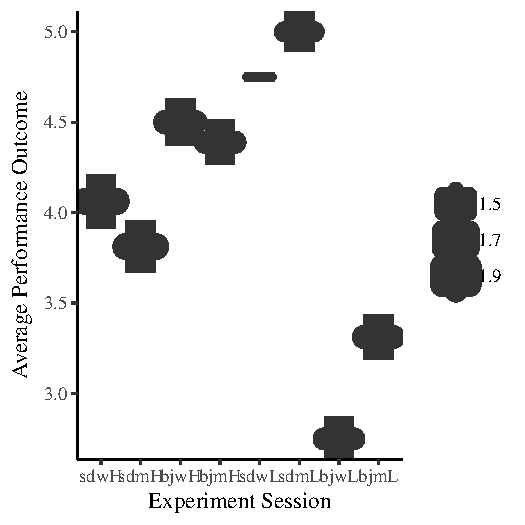
\includegraphics[width=0.5\linewidth,keepaspectratio] {images/fullOutcomeAvgSessionBoxplot-1}%
%  \label{fig:fullOutcomeAvgSessionBoxplot}
%  \caption{Average performance outcome by condition}
%\end{figure}




\subsubsection{Pre-Post Drill survey}
The Pre-Post Drill survey data showed similar results.
There was no significant variation in predictor variables (change in group performance relative to prior expectations, change in individual performance relative to prior expectations, change in perception of components of group or individual performance) according to experiment condition (see Appendix ~\ref{app9:trainingExperiment} Section ~\ref{app9:conditionDifferencesIV} for a full description results).  Similarly, outcome variables (change in team click, change in group bonding, and bonding to team (Province) according to condition) did not vary by condition (see Appendix ~\ref{app9:trainingExperiment} Section ~\ref{app9:manipulationChecksDV} for a full description of results).


These results suggest that there were no clear observable variation in athlete self-report scores according to condition.  Survey responses were collapsed into one overall sample, and condition was introduced as an interaction effect in subsequent LMER models, to investigate the possibility that condition moderated relationships between joint action, team click, and social bonding.














\section{Analysis of Study Predictions\label{sect:resultsStudyPredictions}}

%The high difficulty prime was designed to encourage athletes to 1) generate lower expectations for individual and group performance, and 2) pay closer attention to the details of joint action between participants.  It was predicted that athletes in the high difficulty condition would report more positive perceptions of performance relative to prior expectations.





\subsubsection{Prediction 1: More positive perceptions of team performance relative to prior expectations predict higher feelings of team click with the training group}

\myparagraph{Post-Drill survey}
Results of the Post-Drill survey supported this prediction. There was a significant main effect of Group performance Vs Expectations on Team Click ($\betavec .57 \CIstart .23, .90 \CIfinish \SE .17, t(5.40) = 3.21, \pvalue .02$), indicating that more positive perceptions of group performance relative to prior expectations predicts feelings of team click.  All other main effects were not significant.

Condition was included in the model as an interaction.  Results of the new model revealed a significant positive interaction effect of group performance expectation violation and condition on team click ($\betavec .41 \CIstart .07, .75 \CIfinish \SE .17, t(53) = 2.39, \pvalue .02 $).  A chi-squared test of model fit (based on assessment of AIC value for each nested model) was significant ($\chi^2 (2, N = 53) = 9.42, p = .009$), suggesting that the model in which the interaction effect featured offered a more appropriate fit of the data (for a visualisation of the results, see Figure ~\ref{fig:teamPerfExpClickScatter}).

\begin{figure}
    \centering
    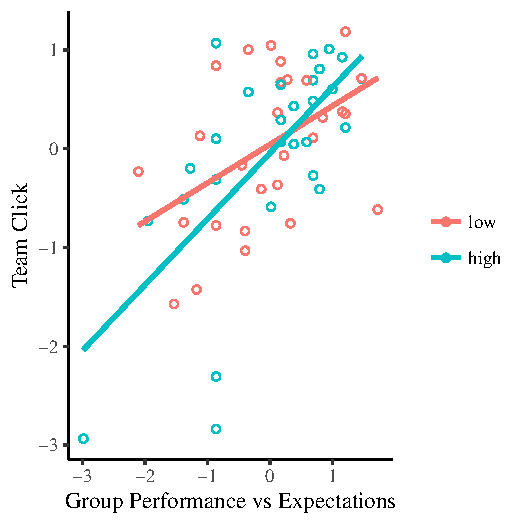
\includegraphics[width=0.5\linewidth,keepaspectratio] {images/teamPerfExpClickScatter-1}
    \caption{More positive perceptions of group performance relative to prior expectations predict team click ($n = 53$).  Both  variables are normalised with mean of zero and SD of one.}
    \label{fig:teamPerfExpClickScatter}
\end{figure}

Model residuals were normally distributed around zero ($\resdist .99, \pvalue .97 $) and an analysis of Cook's distances suggests that the model did not contain any observations that unjustifiably influenced parameter estimates (all $\cooksD < .5$), for full presentation of model assumptions, see Appendix Figure ~\ref{fig:M1Assumptions}).

These results suggest that more positive perceptions of group performance relative to prior expectations predicted stronger feelings of team click, and that perceptions of group performance vs expectations had a greater effect on feelings of team click in the high difficulty condition than in the low difficulty condition.


%Results were in line with predictions that more positive perceptions of group performance relative to prior expectations predicted stronger feelings of team click, an effect observed to be strongest in the high difficulty condition.
%The main effect of condition ($\betavec .76 \CIstart .12, 1.4 \CIfinish \SE .33, t(53) = 2.32, \pvalue .02 $) and group performance expectation violation on feelings of team click with the training group ($\betavec .32 \CIstart .06, .57 \CIfinish, \SE .13, t(53)= 2.41, \pvalue .02$) were also significant.
%The average performance outcome of each Invasion Drill trial was also a significant positive predictor of team click ($\betavec .73 \CIstart .23, 1.24 \CIfinish \SE .26, t(53)= 2.86, \pvalue .006$ (see Table ~\ref{tab:M1lmer}). This result suggested that on-field performance influenced athlete perceptions of performance and team click.



\myparagraph{Pre- to Post-Drill survey}
Results of the Pre- to Post-Drill survey also supported this prediction.  There was a significant main effect of change in perceptions of group performance on change in team click ($\betavec .54 \CIstart .30, .78 \CIfinish \SE .12, t(53) = 4.371, \pvalue .00006$), indicating that greater positive change in perceptions of group performance relative to prior expectations predicts positive change in feelings of team click.  All other main effects were not significant.

Results of a nested model---with condition included as an interaction---revealed a significant positive interaction effect of changes in group performance and condition on team click ($\betavec .47 \CIstart .04, .90 \CIfinish \SE .22, t(53) = 2.16, \pvalue .04 $).  While the interaction effect is clearly identifiable visually (see Figure ~\ref{fig:teamPerfExpClickScatter}),
a chi-squared test of model fit was not significant ($\chi^2 (5, N = 53) = 4.49, p = .48$), suggesting that the model in which the interaction effect featured did not offer a more appropriate fit of the data.

 \begin{figure}
     \centering
     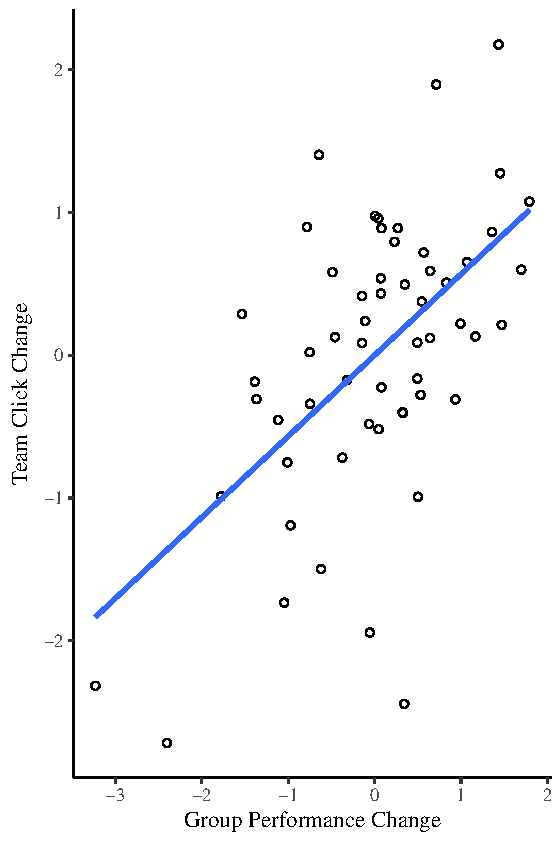
\includegraphics[width=0.5\linewidth,keepaspectratio] {images/groupPerfClickChangeCondition}
     \caption{Change in group performance predicts change in team click ($n = 53$).  Both variables are normalised as z-scores with mean of zero and SD of one.}
     \label{fig:groupPerfClickChangeCondition}
 \end{figure}

Model residuals were normally distributed around zero ($\resdist .98, \pvalue .44$) and an analysis of Cook's distances suggests that the model did not contain any observations that unjustifiably influenced parameter estimates (all $\cooksD < .34$), for full presentation of model assumptions, see Appendix ~\ref{app9:trainingExperiment} Figure ~\ref{fig:M21Assumptions}).

Results suggested that change in perceptions of group performance were a positive predictor of increase in feelings of team click following the Drill.  This relationship is moderated by condition, such that the relationship between change in group performance and team click was stronger in the high difficulty condition.

Results were in line with the prediction that more positive perceptions of group performance relative to prior expectations predicts feelings of team click.



%An LMER, with change in perceptions of group performance, condition, and their interaction included in the model as fixed effects, revealed a significant positive interaction effect of group performance vs expectations and condition on team click ($\betavec .49 \CIstart .06, .92 \CIfinish \SE .22, t(53) = 2.22, \pvalue .03 \MR \CR $).
%The main effect of change in group performance expectation on change in team click was also (highly) significant, ($\betavec .76 \CIstart .46, 1.06 \CIfinish \SE .15, t(53) = 5.018, \pvalue .00006 $). The main effect of condition, however, was not significant ($\betavec .08 \CIstart -.69, .85 \CIfinish \SE .39, t(53) = .20, \pvalue .84 $).
%These results---visualised in figure ~\ref{fig:groupPerfClickChangeCondition}---

%Model residuals were normally distributed around zero ($\resdist .98, \pvalue .45$) and an analysis of Cook's distances suggests that the model did not contain any observations that unjustifiably influenced parameter estimates (all $\cooksD < .34$), for full presentation of model assumptions, see Appendix Figure ~\ref{fig:M1PrePostAssumptions}).





\subsubsection{Prediction 2: Feelings of team click predict feelings of social bonding to the training group}



\myparagraph{Post-Drill survey}
Results of the Post-Drill survey supported this prediction. The model revealed a significant main effect of feelings of team click on feelings of social bonding to the training group ($\betavec .63 \CIstart .46, .79 \CIfinish \SE .09, t(53) = 7.28, p < .0001$), indicating that stronger feelings of team click predict stronger feelings of social bonding.  All other main effects of the model (included as controls) were not significant.

Model residuals were normally distributed around zero ($\resdist .99, \pvalue .80$) and there were no unjustifiably influential cases (all $\cooksD < .6$, see model assumptions in Figure ~\ref{fig:M2Assumptions} in Appendix ~\ref{app9:trainingExperiment} Section ~\ref{app9:postExperimentModelAssumptions}).

These results suggest that athletes who felt stronger levels of team click also felt stronger levels of social bonding to their training group.

%Results of a model in which condition was included as an interaction revealed that the interaction effect of team click and condition on social bonding was not significant, ($\betavec .23 \CIstart -.08, .60 \CIfinish \SE .17, t(23.33) = 1.35, \pvalue .19$).  A chi-squared test of model fit also indicated that the model did not explain the variance with any more precision as the initial model, ($\chi^2 (5, N = 53) = 1.78, p = .88$). These results were confirmed by their visual representation, in which an interaction effect is not obvious (see Figure ~\ref{fig:groupClickBondScatter}).  Thus, the initial model was adopted as the best fit for the data.


\begin{figure}
  \centering
    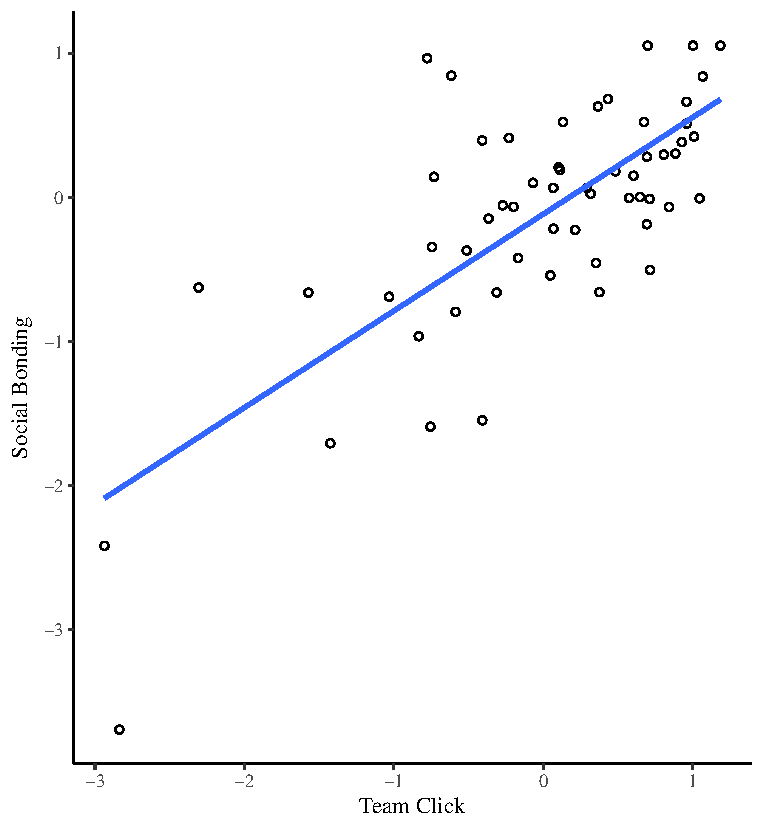
\includegraphics[width=0.5\linewidth,keepaspectratio] {images/groupClickBondScatter}
    \label{fig:groupClickBondScatter}
    \caption{Perceptions of team click predict feelings of social bonding to training group ($n = 53$).  Team click and social bonding are normalised factors ($mean = 0, SD = 1$).}
\end{figure}




%a significant positive interaction effect of group performance expectation violation and condition on team click ($\betavec .41 \CIstart .07, .75 \CIfinish \SE .17, t(53) = 2.39, \pvalue .02 $).  A chi-squared test of model fit (based on assessment of AIC value for each nested model) was significant ($\chi^2 (2, N = 53) = 9.42, p = .009$), suggesting that the model in which the interaction effect featured offered a more appropriate fit of the data (for a visualisation of the results, see Figure ~\ref{fig:teamPerfExpClickScatter}).

%A LMER model in which team click, condition, and their interaction were included as fixed effects, revealed a strong positive relationship between feelings of team click and feelings of social bonding to the training group, $\betavec .43 \CIstart .15, .72 \CIfinish \SE .14, t(29.22) = 2.96, \pvalue .006, \MR , \CR $.
%The main effect of condition ($\betavec .13 \CIstart .15, .72 \CIfinish \SE .29, t(18.7) = 3.15, \pvalue .006$) and the interaction effect of team click and condition on social bonding ($\betavec .26 \CIstart -0.08, .60 \CIfinish \SE .17, t(30.43) = 1.51, \pvalue .14$) were not significant.  These results did, however, appear to be trending in the predicted direction, whereby the relationship between click and bonding appeared stronger in the high difficulty condition.




\myparagraph{Pre- to Post-Drill survey}

Results of the Pre- to Post-Drill survey also offered support for this prediction.  A LMER revealed a significant main effect of change in feelings of team click on change in feelings of social bonding to the training group ($\betavec .27 \CIstart .01, .54 \CIfinish \SE .13, t(53) = 2.05, p < .05$), such that an increased change in team click predicted an increased change in social bonding.  All other main effects of the model were not significant.

Results of a model in which condition was included as an interaction revealed a significant interaction effect of team click and condition on social bonding, ($\betavec .82 \CIstart .38, 1.25 \CIfinish \SE .22, t(47.58) = 3.69, \pvalue .0006$).  A chi-squared test of model fit indicated that the model explained the variance with any more precision than the initial model, ($\chi^2 (5, N = 53) = 11.35, p = .04$).  Graphing the interaction effect clearly demonstrates the extent of the effect (see Figure ~\ref{fig:groupClickBondScatter}).

Model residuals of this second model were normally distributed around zero ($\resdist .96, \pvalue .08$), and Cook's Distances were less than $.5$, indicating that the model did not to contain any observations that unjustifiably influenced parameter estimates (for full presentation of model assumptions, see Figure ~\ref{fig:M22Assumptions} in Appendix ~\ref{app9:trainingExperiment} Section ~\ref{app9:prePostExperimentModelAssumptions}).




\begin{figure}
  \centering
    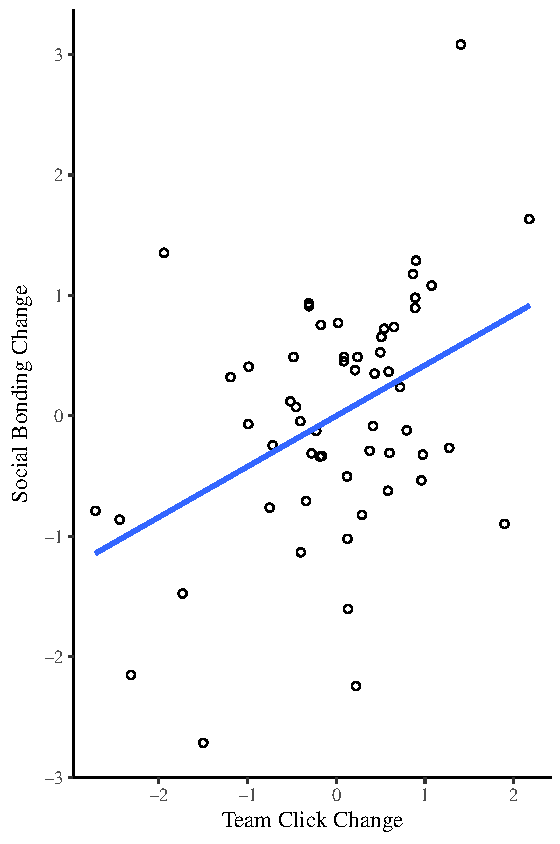
\includegraphics[width=0.5\linewidth,keepaspectratio] {images/groupClickBondingChangeCondition}
    \label{fig:groupClickBondingChangeCondition}
    \caption{Change in perceptions of team click predict change in feelings of social bonding to training group, moderated by condition ($n = 53$)}
\end{figure}

In contrast to the Post-Drill data, the Pre-Post Data revealed not  only a main effect of (change in) team click on (change in) social bonding, but also an interaction effect with condition; the effect of team click on social bonding was more pronounced in the high difficulty condition than the low difficulty condition.


%A LMER model revealed a significant interaction effect of change in team click and experiment condition on change social bonding, ($\betavec .76 \CIstart .32, 1.19 \CIfinish \SE.22, t(47.05) = 3.41, \pvalue .001, \MR , \CR $).  The main effect of change in team click was also a significant predictor of change in social bonding, ($\betavec .58 \CIstart .32, .84 \CIfinish \SE.13, t(40.03) = 4.36, p < .0001 $).  The main effect of condition was not significant, ($\betavec .03 \CIstart -.79, .84 \CIfinish \SE.41, t(17.66) = .06, p < .95 $).  A scatter plot shows that the relationship between change in team click and change in bonding is most pronounced in the high difficulty condition (see figure ~\ref{fig:groupClickBondingChangeCondition}).













\subsubsection{Prediction 3: More positive violations of team performance expectations will predict higher levels of social bonding to the training group}


\myparagraph{Post-Drill survey}
Results generally supported this prediction.  A LMER model revealed that the main effect of group performance vs expectations on social bonding was not significant, ($\betavec .25 \CIstart -.10, .59 \CIfinish \SE .18, t(5.21) = 1.39, \pvalue .22$).  The only significant main effect of the model was arousal, ($\betavec .23 \CIstart .01, .44 \CIfinish \SE .11, t(39.37) = 2.10, \pvalue .04$), suggesting that reports of higher arousal at the end of the drill predict social bonding.  These results did not directly support the prediction that more positive violations of expectations around group performance would also predict higher levels of social bonding.

However, a second model with condition included as an interaction revealed a significant interaction between group performance expectations and condition on social bonding, ($\betavec .44 \CIstart .08, .81 \CIfinish \SE .18, t(53) = 2.41, \pvalue .02$).  A chi-squared test of model fit indicated that the model explained the variance with any more precision than the initial model, ($\chi^2 (2, N = 53) = 6.75, p = .03$).  Graphing the interaction effect clearly demonstrates the extent of the effect (see Figure ~\ref{fig:groupPerfExpBondConditionScatter}).

Model residuals of this second model were normally distributed around zero ($\resdist .97, \pvalue .31$), and Cook's Distances were less than $.6$, indicating that the model did not to contain any observations that unjustifiably influenced parameter estimates (for full presentation of model assumptions, see Figure ~\ref{fig:M3Assumptions} in Appendix ~\ref{app9:trainingExperiment}).

\begin{figure}
  \centering
  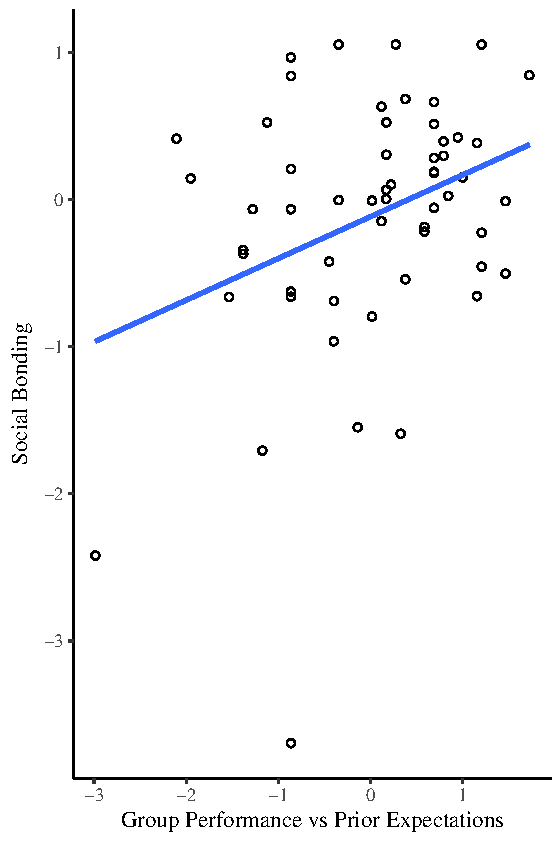
\includegraphics[width=0.5\linewidth,keepaspectratio] {images/groupPerfExpBondConditionScatter}
  \caption{Positive violation of group performance expectations
 predict feelings of social bonding to training group}
 \label{fig:groupPerfExpBondConditionScatter}
\end{figure}



%Average performance in each trial was also a significant predictor of social bonding, $\betavec .65 \CIstart .11, 1.19 \CIfinish \SE .27, t(53) = 2.37, \pvalue .02$. The main effects of group performance vs expectations ($\betavec .008  \CIstart -.27, .28 \CIfinish \SE .14, t(53) = .06, \pvalue .96$) and condition ($\betavec .56  \CIstart 1.12, 1.25 \CIfinish \SE .35, t(53) = 1.6, \pvalue .11$) were not significant. The result for the fixed effect of condition did, however, appear to be trending in the predicted direction ($p = .11$). These results indicate that the the relationship between group performance expectations vs expectations and social bonding was significant only in the high difficulty condition, as demonstrated visually in figure ~\ref{fig:groupPerfExpBondConditionScatter}. Model residuals were normally distributed around zero ($\resdist .97, \pvalue .31, and all \cooksD < .55$, see model assumptions in Appendix  ~\ref{fig:M3Assumptions}).  These results suggested that the relationship between positive violation of group performance expectations and social bonding was significant, only in the high difficulty condition, and not overall across conditions.




\myparagraph{Pre- to Post-Drill survey}


Models of the Pre- to Post-Drill data also produced similar results.  A LMER model revealed that the main effect of change in group performance on change in social bonding was not significant, ($\betavec -0.03 \CIstart -.44, .39 \CIfinish \SE .21, t(7.57) = -.12, \pvalue .91$). The model did reveal a signifiant main effect of change in individual performance on change in social bonding, ($\betavec .28 \CIstart .02, .55 \CIfinish \SE .13, t(49.39) = 2.13, \pvalue .04$), suggesting that more positive increase in perceptions of individual performance predicted more positive increase in social bonding between Pre- and Post-Drill surveys.  However, these results did not directly support the prediction that more positive violations of expectations around group performance would predict higher levels of social bonding.

A second model with condition included as an interaction revealed a significant interaction between group performance expectations and condition on social bonding, ($\betavec .92 \CIstart -1.38, -.48 \CIfinish \SE .23, t(53) = 4.04, \pvalue .0002$).  A chi-squared test of model fit indicated that the model explained the variance with any more precision than the initial model, ($\chi^2 (5, N = 53) = 11.00, p = .05$).  Graphing the interaction effect clearly demonstrates the interaction effect (see Figure ~\ref{fig:groupPerfExpBondConditionScatter}).

Model residuals of this second model were normally distributed around zero ($\resdist .98, \pvalue .55$), and Cook's Distances were less than $.3$, indicating that the model did not to contain any observations that unjustifiably influenced parameter estimates (for full presentation of model assumptions, see Figure ~\ref{fig:M23Assumptions} in Appendix ~\ref{app9:trainingExperiment}).

\begin{figure}
  \centering
  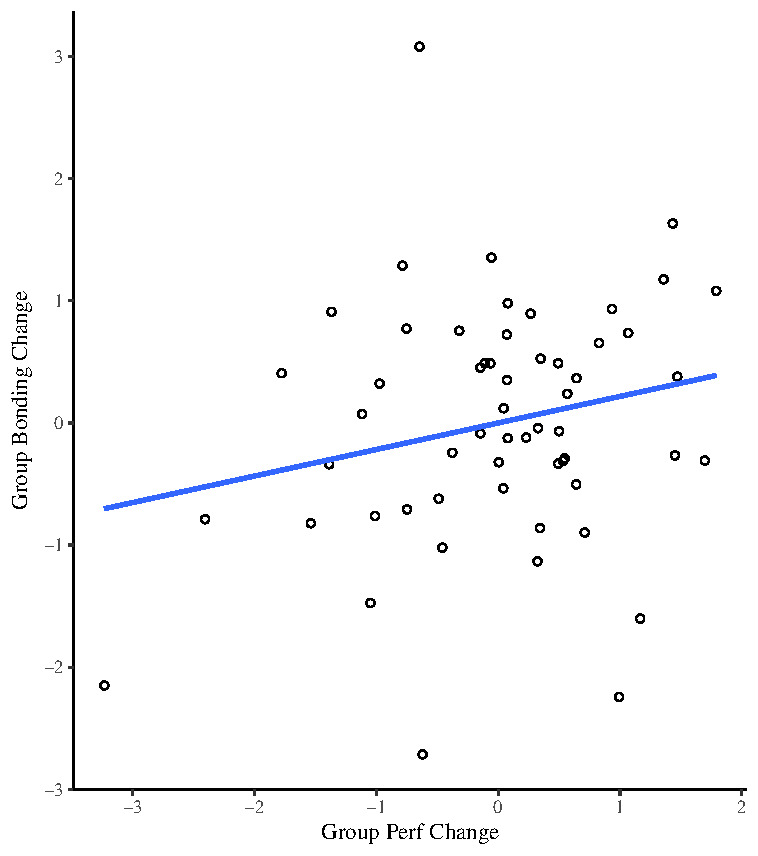
\includegraphics[width=0.5\linewidth,keepaspectratio] {images/groupPerfBondingChangeCondition}
  \caption{Change in perceptions of group performance predict change in social bonding to the training group, only in the high difficulty condition ($n = 53$).  }
 \label{fig:groupPerfBondingChangeCondition}
\end{figure}

These results suggested that the relationship between group performance vs expectations and social bonding was only significant only in the high difficulty condition.


%The interaction effect of change in perceptions of group performance and condition significantly predicted variation in change in social bonding, ($\betavec .49 \CIstart .46, 1.38  \CIfinish \SE .53, t(53) = 4.03, \pvalue .0001, \MR , \CR $). The main effect of change in group performance was also significant, ($\betavec .21  \CIstart .16, .78 \CIfinish \SE.23, t(53) = 2.33, \pvalue .02$), as was the main effect of change in perceptions of individual performance, ($\betavec .26  \CIstart .02, .50 \CIfinish \SE.12, t(53) = 2.15, \pvalue .04$).
%For a full report of model statistics, see APPENDIX ~\ref{tab:M2PrePostOutput}.  This model suggested that the relationship between group performance expectations vs expectations and social bonding was significant only in the high difficulty condition, as demonstrated visually in figure ~\ref{fig:groupPerfExpBondConditionScatter}.

%Model residuals were normally distributed around zero (\resdist .97, \pvalue .31) and all $\cooksD < .22$, see figure ~\ref{fig:M23Assumptions} Appendix ~\ref{app9:trainingExperiment}).   For a full report on tests of model assumptions, see APPENDIX ~\ref{fig:M23Assumptions}.









\subsubsection{Prediction 4: Feelings of team click will mediate a relationship between more positive violations of expectations around group performance and social bonding to the group}


\myparagraph{Post-Drill survey}
The relationship between perceptions of group performance relative to prior expectations and social bonding was mediated by team click and moderated by condition.  LMER models used in analysis of predictions 1 to 3 in the Pre- to Post-Drill survey data were used to construct a mediation model.  Results of the mediation analysis revealed significant average indirect effect of perceptions of group performance relative to prior expectations on social bonding attributable to team click, ($\beta = .30, 95\% CI = .14 , .50, p < .0001$).  When controlling for the effect of team click on social bonding, the average direct effect between group performance vs expectations (moderated by condition) and social bonding was no longer significant ($\beta = -.108, 95\% CI = -.44 , .23, p = .53$, which suggested that a full mediation had occurred (see Figures ~\ref{fig:postExperimentModMedFigure} and ~\ref{fig:groupPerfExpClickChangeMedPlot}).

An analysis of the mediation model according to condition reveals that the mediation effect is moderated by condition.  The mediation effect attributable to the high difficulty condition was more pronounced than the overall effect ($\beta = .52, 95\% CI = .24 , .87, p < .0001$), whereas the mediation effect attributable to the low difficulty condition was not significant, ($\beta = .09, 95\% CI = -.08 , .30, p = .32$, see Figure ~\ref{fig:groupPerfClickChangeMedPlotHighLow} in which the mediation effect is compared by condition).

These results suggest that feelings of team click fully mediated the relationship between perceptions of group performance vs expectations and social bonding, and that this effect was moderated by experiment condition.  The mediating role of team click is driven by results in the high difficulty condition.


\begin{figure}
  \centering
  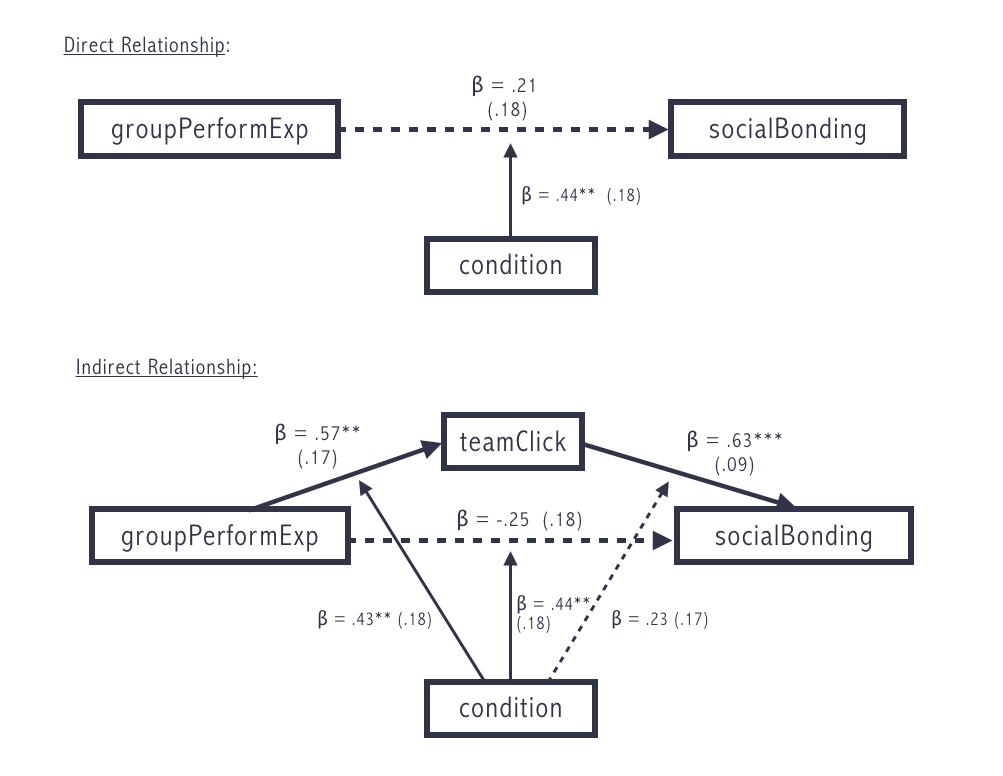
\includegraphics[width=0.9\linewidth,keepaspectratio] {images/modMedPost}
  \caption{Partially moderated full mediation model: team click fully mediates the relationship between group performance and social bonding.  This effect is partially moderated by condition (high).}
  \label{fig:postExperimentModMedFigure}
\end{figure}

\begin{figure}
  \centering
  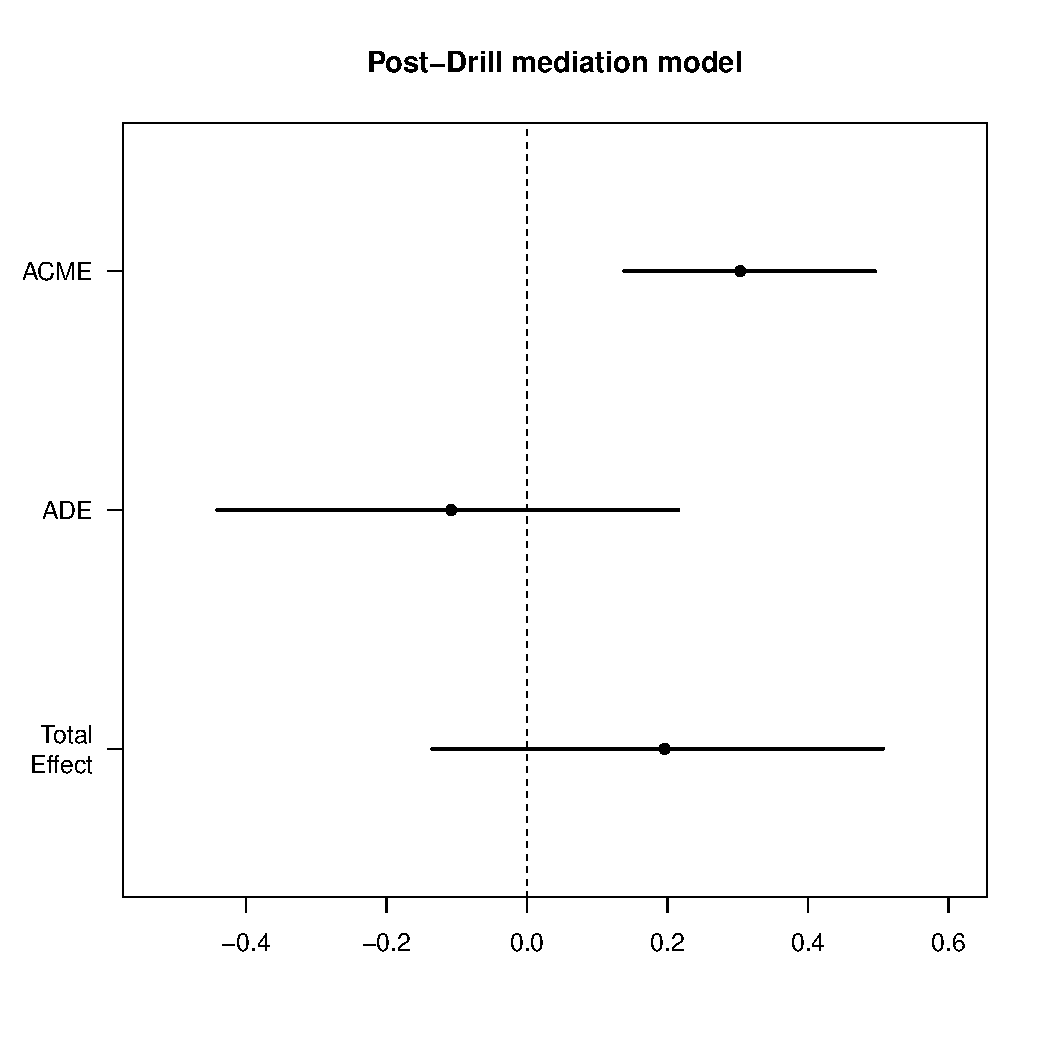
\includegraphics[width=0.5\linewidth,keepaspectratio] {images/groupPerfExpClickMediationPlot}
  \caption{Change in team click fully mediates relationship between team performance expectation violation and social bonding. ACME = Average conditional mediation effect; ADE = Average direct effect.}
  \label{fig:groupPerfExpClickChangeMedPlot}
\end{figure}

\begin{figure}
  \centering
  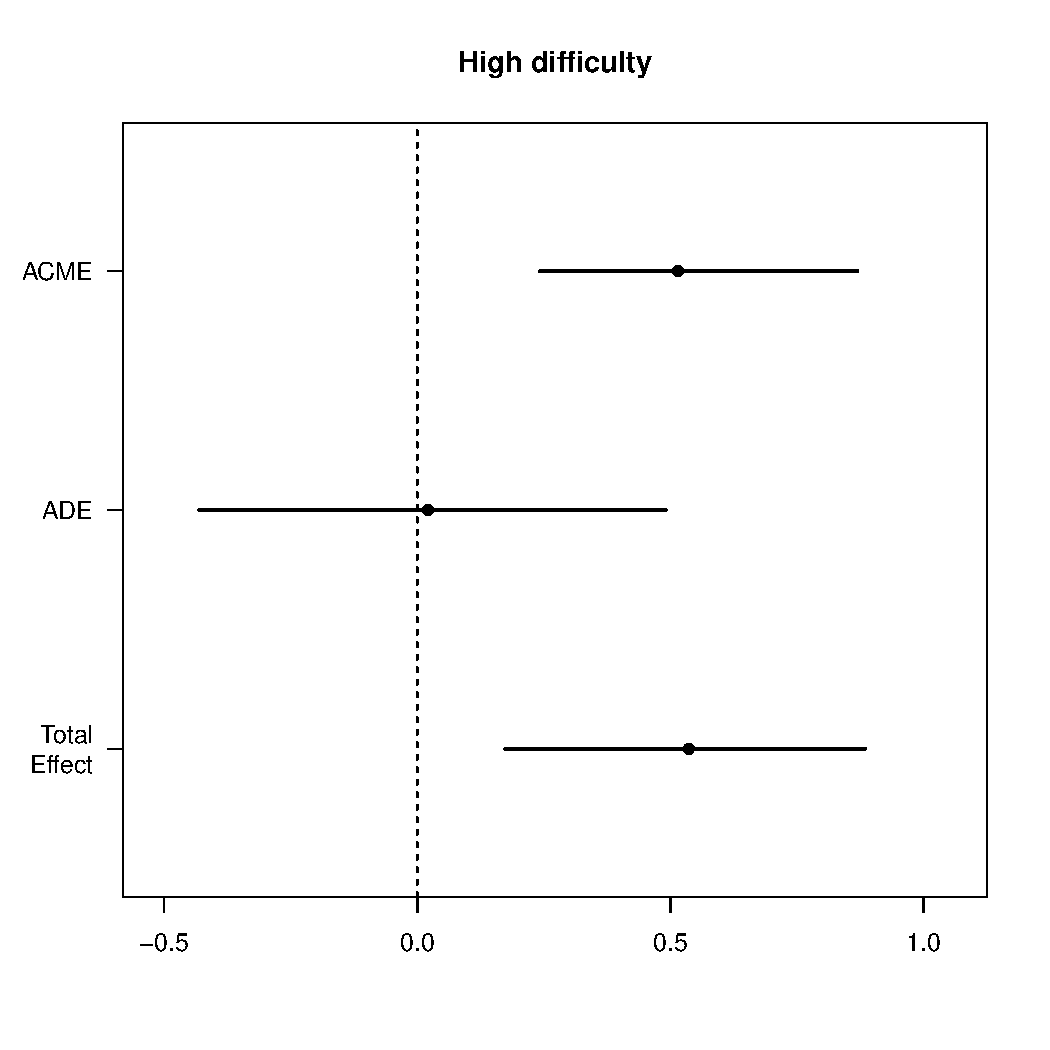
\includegraphics[width=0.3\linewidth,keepaspectratio] {images/groupPerfExpClickMediationPlotHigh}
  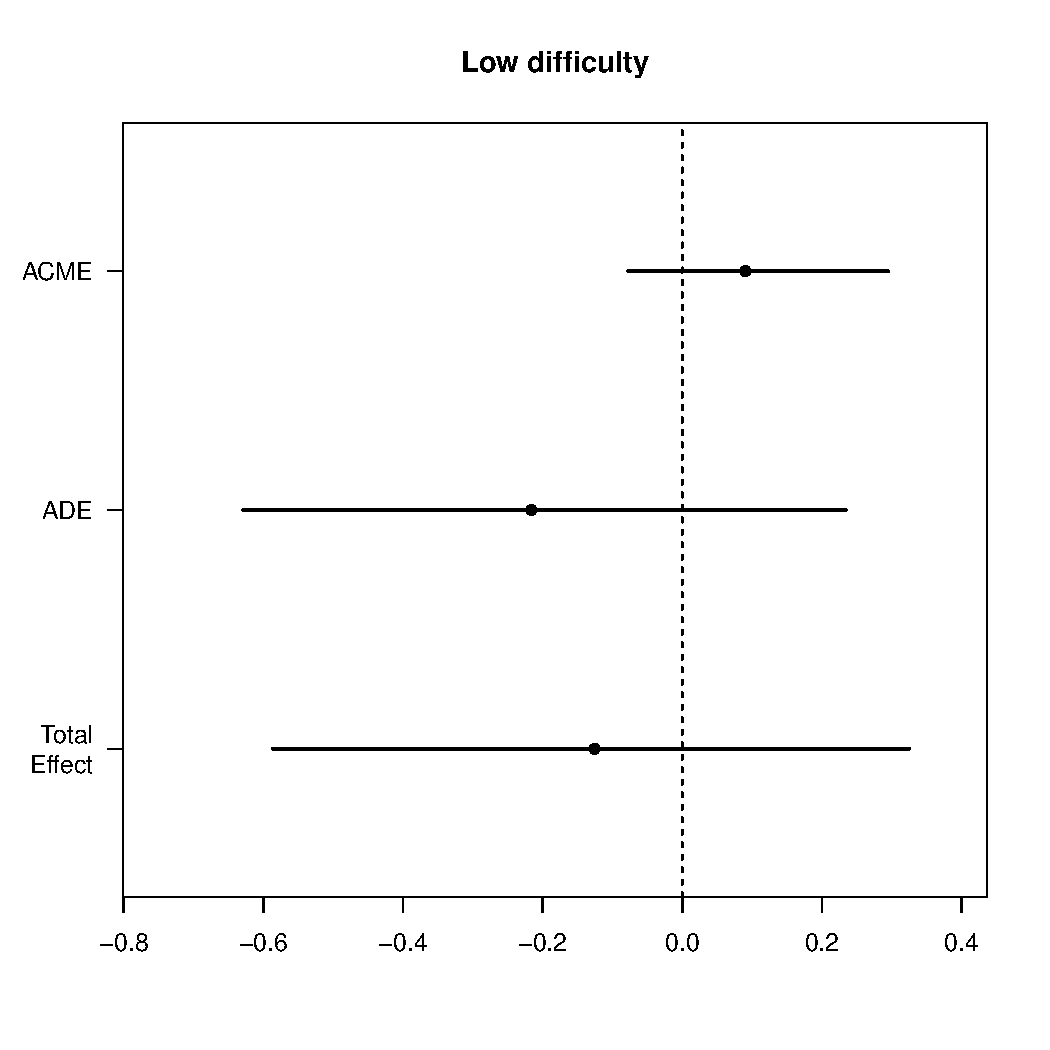
\includegraphics[width=0.3\linewidth,keepaspectratio] {images/groupPerfExpClickMediationPlotLow}
  \caption{Team click mediates relationship between group performance vs expectation and social bonding to the training group in the high difficulty condition, but not the low difficulty condition}
  \label{fig:groupPerfClickChangeMedPlotHighLow}
\end{figure}



\myparagraph{Pre- to Post-Drill survey}

The relationship between change in perceptions of group performance and change in social bonding was mediated by change in team click, and moderated by condition.  LMER models used in analysis of predictions 1 to 3 in the Pre- to Post-Drill survey data were used to construct a mediation model.  Results of the mediation analysis revealed significant average indirect effect of change in perceptions of group performance on change in social bonding attributable to change in team click, ($\beta = .10, 95\% CI = .02, .20, p = .02$).  When controlling for the effect of change in team click on change in social bonding, the average direct effect between change in perceptions of group performance (moderated by condition) and change in social bonding was no longer significant ($\beta = -.10, 95\% CI = -.24 , .05, p = .18$, which suggested that a full mediation had occurred (see Figures ~\ref{fig:prePostExperimentChangeModMedFigure} and ~\ref{fig:groupPerfExpClickChangeMedPlot}).


An analysis of the mediation model according to condition reveals that the mediation effect is moderated by condition.  The mediation effect attributable to the high difficulty condition was more pronounced than the overall effect ($\beta = .21, 95\% CI = .07 , .38, p = .004$), whereas the mediation effect attributable to the low difficulty condition was not significant, ($\beta = -.01, 95\% CI = -.09 , .04, p = .67$), see Figure ~\ref{fig:groupPerfClickChangeMedPlotHighLow} in which the mediation effect is compared by condition).

%The average direct ($\beta = -.21, 95\% CI = -.09 , .04, p = .67$) and total ($\beta = -.21, 95\% CI = -.09 , .04, p = .67$)effects of this model were significant,

These results suggest that positive increase in feelings of team click after the Drill fully mediated a relationship between a positive increase in perceptions of group performance and a positive increase in feelings of social bonding to the training group. This mediation effect was moderated by experiment condition, such that the mediating role of team click is driven by results in the high difficulty condition.


\begin{figure}
  \centering
  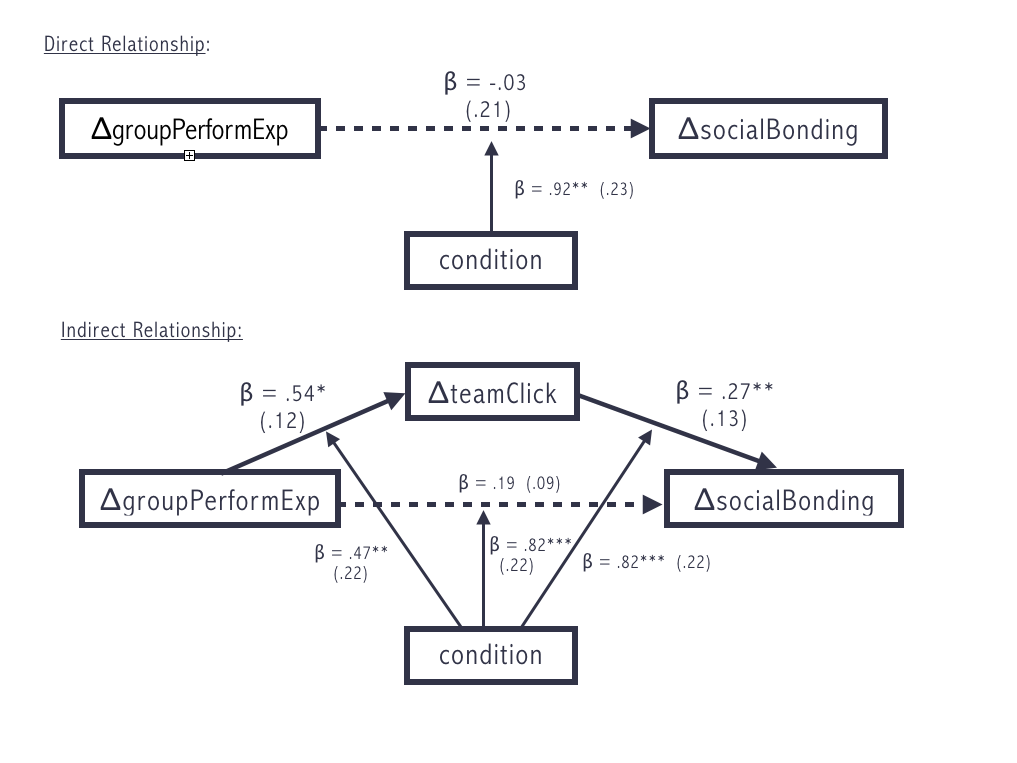
\includegraphics[width=0.9\linewidth,keepaspectratio] {images/modMedChangePrePost}
  \caption{Moderated mediation model: team click mediates the realtionship between group performance and social bonding.  This effect is partially moderated by condition (high).}
  \label{fig:prePostExperimentChangeModMedFigure}
\end{figure}

\begin{figure}
  \centering
  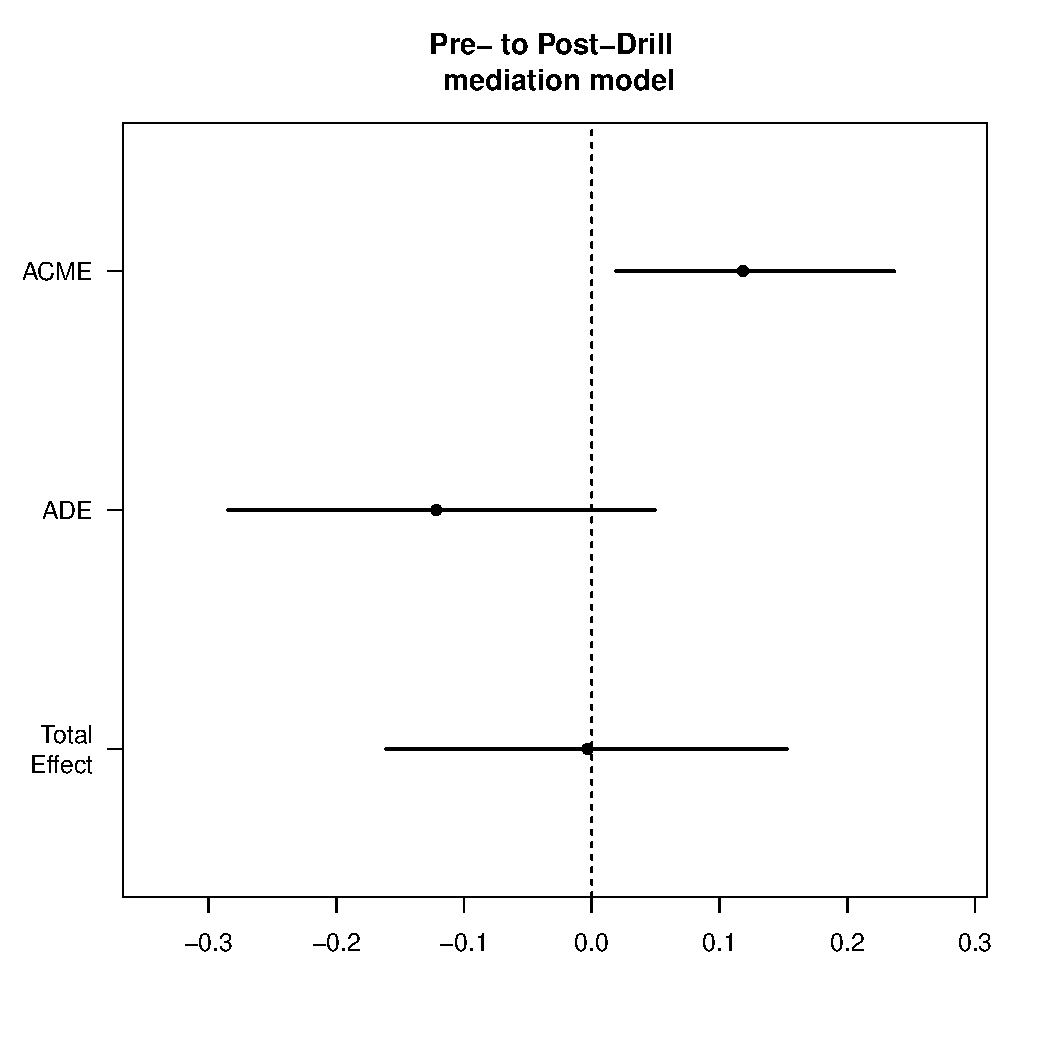
\includegraphics[width=0.5\linewidth,keepaspectratio] {images/groupPerfExpClickChangeMedPlot}
  \caption{Change in team click partially mediates relationship between group performance vs expectation and social bonding ($n = 53$)}
  \label{fig:groupPerfExpClickChangeMedPlot}
\end{figure}

\begin{figure}
  \centering
  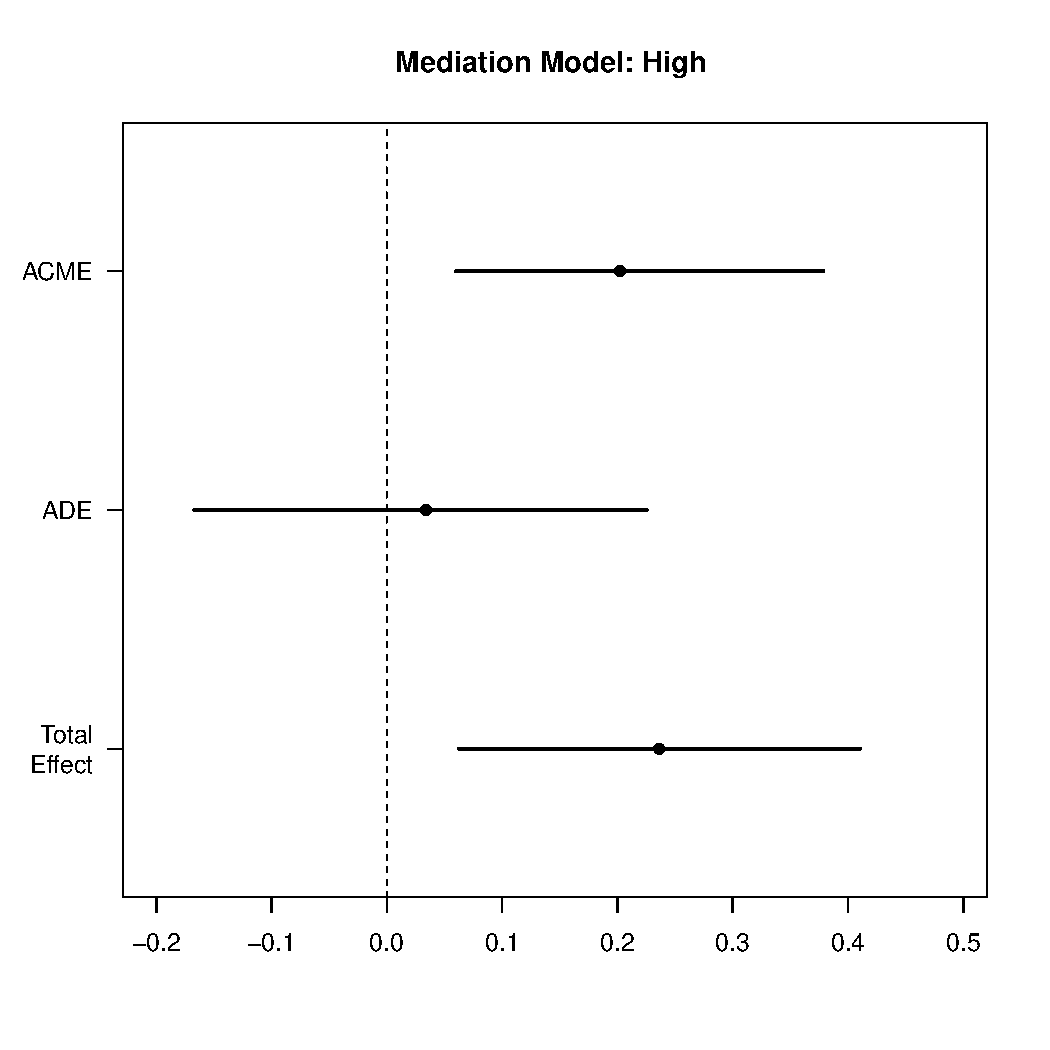
\includegraphics[width=0.3\linewidth,keepaspectratio] {images/groupPerfClickChangeMedPlotHigh}
  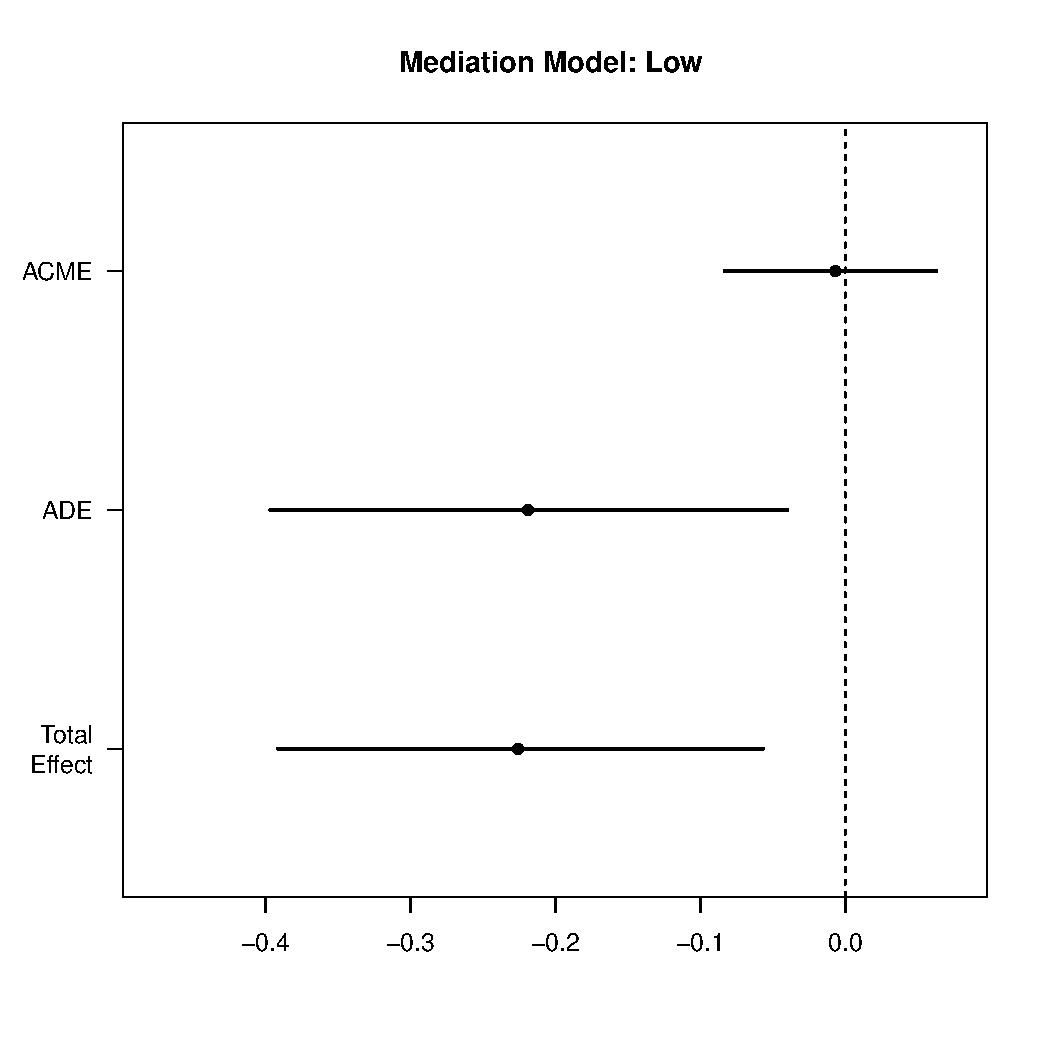
\includegraphics[width=0.3\linewidth,keepaspectratio] {images/groupPerfClickChangeMedPlotLow}
  \caption{Change in team click fully mediates a relationship between change in group performance and change in social bonding, only in the high difficulty condition ($n = 53$)}
  \label{fig:groupPerfClickChangeMedPlotHighLow}
\end{figure}










%Results of the mediation analysis revealed significant average indirect effect of change in group performance perception on change in social social bonding, attributable to change in team click, $\betavec.09 \CIstart .10, .02  \CIfinish, \pvalue .02$.  When controlling for the effect of team click on social bonding, the average direct effect between Joint Action Success and social bonding was no longer significant, $\betavec -.08  \CIstart -.23, .06 \CIfinish, \pvalue .24$  (see Figure ~\ref{fig:groupPerfExpClickMediationPlot}).

%Closer analysis revealed that the mediation was moderated by experiment condition: the mediation was significant only for the high difficulty condition ($\betavec .52  \CIstart .24, .87 \CIfinish, p <=.0001$), but not the low difficulty condition, ($\betavec .09  \CIstart -.08, .30 \CIfinish, p =.32$). The moderated mediation model is shown in figure ~\ref{fig:prePostExperimentChangeModMedFigure}, and the overall and moderated mediation effects are contrasted graphically in figures ~\ref{fig:groupPerfExpClickChangeMedPlot}\nobreakdash~\ref{fig:prePostExperimentChangePlotLow}.  These results suggest that feelings of team click fully mediate the relationship between change in perceptions of group performance and social bonding, only in the high experiment condition.  In a similar fashion to the results of the Post-Drill analysis, results supported predictions that feelings of team click fully mediate a relationship between experience of social bonding and social bonding.





\clearpage
\section{Discussion}
%study:
This study was designed to investigate the social cognition of team click in a controlled field experiment.  Athletes participated in a training drill paradigm in which overt feedback concerning performance was restricted to athletes' perceptions of each phase of the Invasion Drill.  Athletes were not overtly declared as winners or losers, and there was nothing explicit to gain from the experiment---unlike in the high stakes national tournament that was the focus of the previous study (Chapter~\ref{tournamentSurvey}).  Unlike a high stakes rugby tournament, the training drill did not entail high levels of physiological cost, in fact only required low-to-medium level exertion and ``grab'' as opposed to full-contact. Instead, coordination in joint action was isolated as the key component of the experimental paradigm.  Results of this study generally support study predictions, and reproduced the correlational results of the survey study in a more controlled setting. Taken toghether, these empirical studies substantiate ethnographic observations made in the first part of this dissertation, and offer preliminary evidence for a novel theory, outlined in this thesis, of social bonding through joint action in group exercise contexts.



\myparagraph{Summary of results}

Post-Drill generally confirmed predictions by demonstrating positive significant associations between perceptions of performance (relative to prior expectations), team click, and social bonding.  The mediation effect also confirmed that the experience of high quality coordination in joint action (team click) mediated a relationship between joint action and social bonding.  The fact that this result was further moderated by experiment condition suggests that (positive) expectation violation in joint action could be an important explanatory mechanism.  The moderation effect of condition was only significant in the relationship between group performance vs. expectations and team click, however.

%results:
Significant positive relationships between 1) perceptions of performance in joint action relative to prior expectation and team click, 2) team click and social bonding,  and 3) performance in joint action and social bonding were moderated by experiment condition, such that these relationships were strongest in athletes who participated in the high difficulty condition.  Mediation models supported these findings, showing evidence of a moderated mediation effect of team click on the relationship between group performance vs expectations and social bonding.  In both the Post-Drill and pre- to Post-Drill analyses, the mediation effect was moderated by experiment condition: the relationship was either strongest or only present in the high difficulty condition on not in the low difficulty condition.  Despite an overall trend in which scores decreased between pre- and Post-Drill measures, athletes who on average experienced more positive perceptions of performance following the Experiment also reported higher average levels of team click and social bonding (a statistical relationship that was against the overall trend in the data).  The results described here held when statistically controlling for athlete perceptions of individual performance, technical competence, objective performance outcome in the experiment session, and physiological arousal.

\myparagraph{Inferences}
From these results it is possible to infer that perceptions of joint action feature strongly in athletes' formulation of social attitudes, for example feelings of social bonding and group membership.  The experience of higher levels of click in joint action may also be a particularly powerful phenomenon in the formation of positive associations with teammates and team identity.  In addition, results of this study provide some support for the theory, outlined in this dissertations, that the formulation and violation of expectations around joint action is a mechanism of central importance to the social cognition of joint action.  The exhilarating phenomenon of team click in joint action could be associated with positive violations of athletes expectations, which are implicitly formulated and calibrated over time with their teammates in training and competition.  Interactive team sports such as rugby provide a situation in which optimising quality of joint action is the explicit shared goal of the group---the group's reason for being----and so it is understandable that joint action would feature strongly in athlete inferences about group membership.


\myparagraph{Limitations}
Although the experiment manipulation appeared to statistically moderate a relationship between joint action and social bonding, these results were not supported by the study's manipulation checks, all of which did not produce significant results.  The design and execution of the experiment was such that the possibility that the significant moderating effect of condition was the artefact of low sample size and limited randomisation of athlete sampling. The experiment manipulation was subtle, and was delivered by a researcher who spoke Chinese as a second language, perhaps unable to manufacture a sufficient performance Pre-Drill to alter the expectations of athletes. In addition, the limitations of research context, namely time constraints and access to athletes, were such that pilot phase was not exhaustive as it could have been (2 trials per condition).

The experiment sought to isolate expectation violation as a mechanism of central importance to the social cognition of joint action.  While results show evidence for condition-wise effects, in which the high difficulty condition was responsible for moderating the relationship between joint action, team click, and social bonding, it is not sufficiently clear precisely what mechanism drove these results.
The fact that the hypothesised mechanisms of joint action and social bonding have been shown to exist pre-declaratively and predominantly below the surface of conscious experience presents a methodological challenge for psychological research which relies heavily on self-report.



%    [ ] what inferences can we make from these results?
%    [ ] How does it relate to other literature?
%    [ ] limitations
%    [ ] future work —> experiment (takes away explicit feedback)
%    [ ]  "Conclude the general discussion with a strong paragraph stating the main point or points again, in somewhat different terms-if possible-than used before.”
